\batchmode
\makeatletter
\def\input@path{{"C:/Users/tkpme/Dropbox/BookPCRA/Springer Production March 2026/Ch Appendix B Prob & Stat for PCRM/"}}
\makeatother
\documentclass[graybox,envcountchap,sectrefs]{svmono}\usepackage[]{graphicx}\usepackage[]{xcolor}
% maxwidth is the original width if it is less than linewidth
% otherwise use linewidth (to make sure the graphics do not exceed the margin)
\makeatletter
\def\maxwidth{ %
  \ifdim\Gin@nat@width>\linewidth
    \linewidth
  \else
    \Gin@nat@width
  \fi
}
\makeatother

\definecolor{fgcolor}{rgb}{0.345, 0.345, 0.345}
\newcommand{\hlnum}[1]{\textcolor[rgb]{0.686,0.059,0.569}{#1}}%
\newcommand{\hlsng}[1]{\textcolor[rgb]{0.192,0.494,0.8}{#1}}%
\newcommand{\hlcom}[1]{\textcolor[rgb]{0.678,0.584,0.686}{\textit{#1}}}%
\newcommand{\hlopt}[1]{\textcolor[rgb]{0,0,0}{#1}}%
\newcommand{\hldef}[1]{\textcolor[rgb]{0.345,0.345,0.345}{#1}}%
\newcommand{\hlkwa}[1]{\textcolor[rgb]{0.161,0.373,0.58}{\textbf{#1}}}%
\newcommand{\hlkwb}[1]{\textcolor[rgb]{0.69,0.353,0.396}{#1}}%
\newcommand{\hlkwc}[1]{\textcolor[rgb]{0.333,0.667,0.333}{#1}}%
\newcommand{\hlkwd}[1]{\textcolor[rgb]{0.737,0.353,0.396}{\textbf{#1}}}%
\let\hlipl\hlkwb

\usepackage{framed}
\makeatletter
\newenvironment{kframe}{%
 \def\at@end@of@kframe{}%
 \ifinner\ifhmode%
  \def\at@end@of@kframe{\end{minipage}}%
  \begin{minipage}{\columnwidth}%
 \fi\fi%
 \def\FrameCommand##1{\hskip\@totalleftmargin \hskip-\fboxsep
 \colorbox{shadecolor}{##1}\hskip-\fboxsep
     % There is no \\@totalrightmargin, so:
     \hskip-\linewidth \hskip-\@totalleftmargin \hskip\columnwidth}%
 \MakeFramed {\advance\hsize-\width
   \@totalleftmargin\z@ \linewidth\hsize
   \@setminipage}}%
 {\par\unskip\endMakeFramed%
 \at@end@of@kframe}
\makeatother

\definecolor{shadecolor}{rgb}{.97, .97, .97}
\definecolor{messagecolor}{rgb}{0, 0, 0}
\definecolor{warningcolor}{rgb}{1, 0, 1}
\definecolor{errorcolor}{rgb}{1, 0, 0}
\newenvironment{knitrout}{}{} % an empty environment to be redefined in TeX

\usepackage{alltt}
\usepackage{mathptmx}
\usepackage{helvet}
\usepackage{courier}
\usepackage[T1]{fontenc}
\usepackage[utf8]{inputenc}
\usepackage{geometry}
\geometry{verbose,tmargin=1in,bmargin=1in,lmargin=1in,rmargin=1in}
\setcounter{tocdepth}{3}
\setlength{\parskip}{\medskipamount}
\setlength{\parindent}{0pt}
\usepackage{float}
\usepackage{units}
\usepackage{textcomp}
\usepackage{url}
\usepackage{amsmath}
\usepackage{amssymb}
\usepackage{graphicx}
\PassOptionsToPackage{normalem}{ulem}
\usepackage{ulem}
\usepackage[unicode=true,pdfusetitle,
 bookmarks=true,bookmarksnumbered=true,bookmarksopen=true,bookmarksopenlevel=1,
 breaklinks=false,pdfborder={0 0 1},backref=false,colorlinks=false]
 {hyperref}
\hypersetup{
 pdfstartview=XYZ null null 1.25,pdfpagemode=UseNone}

\makeatletter
%%%%%%%%%%%%%%%%%%%%%%%%%%%%%% User specified LaTeX commands.
%%%%%%%%%%%%%%%%%%%% book.tex %%%%%%%%%%%%%%%%%%%%%%%%%%%%%
%
% sample root file for the chapters of your "monograph"
%
% Use this file as a template for your own input.
%
%%%%%%%%%%%%%%%% Springer-Verlag %%%%%%%%%%%%%%%%%%%%%%%%%%


% RECOMMENDED %%%%%%%%%%%%%%%%%%%%%%%%%%%%%%%%%%%%%%%%%%%%%%%%%%%


% choose options for [] as required from the list
% in the Reference Guide

\usepackage{makeidx}% allows index generation
% standard LaTeX graphics tool
                             % when including figure files
\usepackage{multicol}% used for the two-column index
\usepackage[bottom]{footmisc}% places footnotes at page bottom

\usepackage{hyperref}
\def\UrlBreaks{\do\/\do-}

% see the list of further useful packages
% in the Reference Guide

\makeindex             % used for the subject index
                       % please use the style svind.ist with
                       % your makeindex program


%\usepackage[ style=authoryear,natbib=true,giveninits=true,backend=biber,maxcitenames=2]{biblatex}
\usepackage[style=authoryear,natbib=true,firstinits=false,backend=biber,maxcitenames=2]{biblatex}


\setlength{\bibitemsep}{0.5\baselineskip}
\DeclareNameAlias{sortname}{family-given}

\IfFileExists{C:/Users/Doug/Dropbox/BookPCRA/mpslbookCombined.bib}
{\addbibresource[location=local]{C:/Users/Doug/Dropbox/BookPCRA/mpslbookCombined.bib}}
{   \IfFileExists{C:/Users/tkpme/Dropbox/BookPCRA/mpslbookCombined.bib}
    {\addbibresource[location=local]{C:/Users/tkpme/Dropbox/BookPCRA/mpslbookCombined.bib}}
    {   \IfFileExists{C:/Users/stoya/Dropbox/BookPCRA/mpslbookCombined.bib}
        {\addbibresource[location=local]{C:/Users/stoya/Dropbox/BookPCRA/mpslbookCombined.bib}}
        {   \IfFileExists{C:/Users/4thauthor/Dropbox/BookPCRA/mpslbookCombined.bib}
            {\addbibresource[location=local]{C:/Users/4thauthor/Dropbox/BookPCRA/mpslbookCombined.bib}}
            {}
        }
    }
}
\renewcommand\cite{\citet}

\usepackage{amsmath}
\usepackage{amssymb}
\usepackage[p,osf]{stickstootext}
\usepackage[stix2,vvarbb]{newtxmath}
\usepackage[varqu,varl]{inconsolata}
% \usepackage{txfonts}
\usepackage{upgreek}

\DeclareMathOperator{\argmax}{arg\,max}
\DeclareMathOperator{\argmin}{arg\,min}
\usepackage{array}
\usepackage{arydshln}
\usepackage{booktabs}
\usepackage{threeparttablex}
\usepackage{appendix}

\usepackage[utf8]{inputenc}
%%%%%%%%%%%%%%%%%%%%%%%%%%%%%%%%%%%%%%%%%%%
\IfFileExists{C:/Users/Doug/Dropbox/BookPCRA/macroSP_August_05_2021.tex}
{\input{C:/Users/Doug/Dropbox/BookPCRA/macroSP_August_05_2021.tex}}
{   \IfFileExists{C:/Users/tkpme/Dropbox/BookPCRA/macroSP_August_05_2021.tex}
    {\input{C:/Users/tkpme/Dropbox/BookPCRA/macroSP_August_05_2021.tex}}
    {   \IfFileExists{C:/Users/stoya/Dropbox/BookPCRA/macroSP_August_05_2021.tex}
        {\input{C:/Users/stoya/Dropbox/BookPCRA/macroSP_August_05_2021.tex}}
        {   \IfFileExists{C:/Users/4thAuthor/Dropbox/BookPCRA/macroSP_August_05_2021.tex}
            {\input{C:/Users/4thAuthor/Dropbox/BookPCRA/macroSP_August_05_2021.tex}}
            {}
        }
    }
}

\belowsink=90pt

%%%%%%%%%%%%%%%%%%%%%%%%%%%%%%%%%%%%%%%%%%%%%

\makeatother

\providecommand{\examplename}{Example}
\IfFileExists{upquote.sty}{\usepackage{upquote}}{}
\begin{document}
\begin{appendices}


\setcounter{chapter}{1} 

\chapter{PROBABILITY AND STATISTICS FOR PCRA\label{chap:AppendixB}}

\vspace{0.3in}

\textbf{Planned for publication in 2026 by R. Douglas Martin, Thomas
K. Philips, Bernd Scherer and Kirk Li. All rights reserved. © Copyright
2025}

\vspace{0.3in}

\begin{center}
10/12/25
\par\end{center}

\tocchpnum=30pt 
\tocsecnum=33pt 
\tocsubsecnum=40pt 
\tocsubsubsecnum=48pt 
\tocparanum=55pt 
\tocsubparanum=63pt
\calctocindent

\tableofcontents{}\newpage{}

This Appendix contains a variety of probability and statistics results
that are useful the context of portfolio construction and risk management
theory and methods.

\textbf{{*}}

\section{Location and Scale Distributions}

Let $R$ be a random variable (think of $R$ as a return, but it could
be any random variable) with location parameter $\mu$ and scale parameter
$s>0$. The probability distribution function $F_{R}(r)$ and density
function $f_{R}(r)$ of $R$ have the forms

\begin{subequations}
\begin{align}
F_{R}(r) & =F\left(\frac{r\,-\,\mu}{s}\right),\label{eq:LocScaleDistribution}\\[0.5em]
f_{R}(r) & =\frac{1}{s}f\left(\frac{r\,-\,\mu}{s}\right).\label{eq:LocScaleDensity}
\end{align}
\end{subequations}

Roughly speaking, the location parameter tells us where $f_{R}(r)$
is centered, while the scale parameter tells us how widely it spreads.
The most famous member of the location--scale family of distributions
is the Normal distribution, whose density function is
\begin{equation}
f_{R}(r)=\frac{1}{\sqrt{2\pi\sigma^{2}}}\exp\left(-\frac{\left(r-\mu\right)^{2}}{2\sigma^{2}}\right),\ -\infty<r<\infty.\label{eq:NormalDensity}
\end{equation}

The mapping from \eqref{eq:NormalDensity} to \eqref{eq:LocScaleDensity}
is obvious: the location parameter $\mu$ is the mean of the distribution,
and the scale parameter $\sigma$ is the square root of its variance
$\sigma^{2}$. A closely related location-scale family is the family
of t-distributions, with density function
\begin{equation}
f_{R}(r)=\frac{\Gamma\left(\frac{\nu\,+\,1}{2}\right)}{\Gamma\left(\frac{\nu}{2}\right)\sqrt{\pi\,\nu\,\tau^{2}}}\left(1+\frac{1}{\nu}\,\frac{\left(r-\mu\right)^{2}}{\tau^{2}}\right)^{\nicefrac{\left(\nu+1\right)}{2}},\ -\infty<r<\infty.\label{eq:tDensity}
\end{equation}
location parameter $\mu$, and scale parameter $\tau$. For $\nu>1$,
the mean of the distribution is $\mu$, and for $\nu>2$, its variance
is $\tau^{2}\cdot\nicefrac{\nu}{\nu\,-\,2}$. The mean of the t-distribution
is undefined for $\nu=1,$ and its variance is undefined for $\nu\leqslant2$.
In the special case when $\nu=1$, the t-distribution is known as
a Cauchy distribution, and its mean is undefined, even though the
distribution is centered at 0.

A less well-known, but still important, member of the location-scale
family is the Laplacian, or two-sided exponential, distribution with
density function
\begin{equation}
f_{R}(r)=\frac{1}{2b}\exp\left(-\frac{\left|r-\mu\right|}{b}\right),\ -\infty<r<\infty.\label{eq:LaplacianDensity}
\end{equation}
The location parameter $\mu$ is the mean of the distribution, and
the scale parameter $b$ is $\nicefrac{1}{\sqrt{2}}$ times its standard
deviation, or the square root of its variance. The Laplacian distribution
can be shown to be a lateral translation by $\mu$ of the difference
between two exponential random variables with pdf $\nicefrac{\exp\left(\nicefrac{-r}{b}\right)}{\,b}$\footnote{Most textbooks describe the exponential distribution in terms of a
rate parameter $\lambda$ that is the reciprocal of $b$. We deliberately
use $b$ in place of $\lambda$ to emphasize the commonality with
\ref{eq:LocScaleDensity}.}.


\section{Invariance Properties of Location, Scale, Covariance and Correlation}

\subsubsection*{Mean and Standard Deviation Equivariance}

Let $\mu_{R}=\mathrm{E\left[\mathit{R}\right]}$ and $\sigma_{R}=\sqrt{\mathrm{var}(R)}$
be the mean and standard deviation of $R$, and let $\dot{R}$ be
an \emph{affine transformation}\footnote{An affine transformation has both a constant and a linear term --
it is best thought of as a parallel shift of a linear transformation.} of $R$ defined as
\[
\dot{R}=a\,+\,bR
\]
where $a$ is a location parameter and $b>0$ is a scale parameter.
It is straightforward to show that
\begin{align*}
\mu_{\dot{R}} & =a\,+\,b\mu_{R}\\
\sigma_{\dot{R}} & =b\,\cdot\,\sigma_{R}.
\end{align*}
The first equation above shows that the mean is \emph{location and
scale equivariant}, and the second equation shows that the standard
deviation is \emph{location invariant} and \emph{scale equivariant}.

\subsubsection*{Covariance Translation Invariance and Scale Equivariance}

Now suppose that $r_{i}$ and $r_{j}$ have covariance $\mathrm{cov}(r_{i},\,r_{j})$
and assume that variables $\dot{r}_{i}$ and $\dot{r}_{j}$ are obtained
from $r_{i}$ and $r_{j}$ by the affine transformations
\begin{align}
\dot{r}_{i} & =a\,+\,b\,\cdot\,r_{i}\nonumber \\
\dot{r}_{j} & =c\,+\,d\,\cdot\,r_{j}.\label{eq:affineTF}
\end{align}
The resulting covariance, $\mathrm{cov}(\dot{r}_{i},\,\dot{r}_{j})$,
of $\dot{r}_{i}$ and $\dot{r}_{j}$ is
\begin{equation}
\mathrm{cov}(\dot{r}_{i},\,\dot{r}_{j})=b\,\cdot\,d\,\cdot\,\mathrm{cov}(r_{i},\,r_{j}),\label{eq:covAffineTF}
\end{equation}
and we describe this behavior by saying that covariances are \emph{translation
invariant} and \emph{scale equivariant}.

\subsubsection*{Correlation Affine Invariance}

Since the correlation of $r_{i}$ and $r_{j}$ is
\begin{equation}
\mathrm{cor}(r_{i},\,r_{j})=\frac{\mathrm{cov}(r_{i},\,r_{j})}{\sigma_{r_{i}}\,\cdot\,\sigma_{r_{j}}},
\end{equation}
it follows that follows that the correlation of $\dot{r}_{i}$ and
$\dot{r}_{j}$ obtained by the affine transform \eqref{eq:affineTF}
is the same as the correlation between $r_{i}$ and $r_{j}$, namely
\begin{equation}
\mathrm{cor}(\dot{r}_{i},\,\dot{r}_{j})=\mathrm{cor}(r_{i},\,r_{j})\label{eq:corrsAffineInvariance}
\end{equation}
and we see that \emph{correlations are affine invariant}.

\subsubsection*{Corresponding Properties of Sample Estimators}

It is easy to check that the above equivariance and invariance properties
also hold for the sample based estimators

\section{Linearity of Covariances\label{sec: covarianceLinearity}}

Suppose we have two random variables, $x$ and $z$, where $z=\sum_{i\,=\,1}^{n}a_{i}\,y_{i}$.
Then
\begin{eqnarray}
\mathrm{cov}(x,\,z) & = & \mathrm{cov}\left(x,\ \sum_{i\,=\,1}^{n}a_{i}\,y_{i}\right)\nonumber \\
 & = & \mathrm{E}\left[\left(x\,-\,\mathrm{E\left[\mathit{x}\right]}\right)\left(\sum_{i\,=\,1}^{n}a_{i}y_{i}\,-\,\sum_{i\,=\,1}^{n}a_{i}\,\mathrm{E}\left[y_{i}\right]\right)\right]\nonumber \\
 & = & \mathrm{E}\left[\sum_{i\,=\,1}^{n}a_{i}\left(x\,-\,\mathrm{E}\left[x\right]\right)\left(y_{i}\,-\,\mathrm{E}\left[y_{i}\right]\right)\right]\nonumber \\
 & = & \sum_{i\,=\,1}^{n}a_{i}\,\mathrm{E}\left[\left(x\,-\,\mathrm{E}\left[x\right]\right)\left(y_{i}\,-\,\mathrm{E}\left[y_{i}\right]\right)\right]\nonumber \\
 & = & \sum_{i\,=\,1}^{n}a_{i}\,\mathrm{cov}(x,\,y_{i})\nonumber \\
 & = & \mathbf{a^{\prime}}\mathrm{cov}(x,\,\mathbf{y})\label{eq: covLinearity}
\end{eqnarray}
where $\mathrm{cov}(x,\,\mathbf{y})$ is an $n$--dimensional column
vector with $i^{th}$ element $\mathrm{cov}(x,\,y_{i})$.

A leading application of the above covariance linearity property is
the computation of the covariance between the return of a portfolio,
$r_{P}$, and its $i^{th}$ constituent asset, $r_{i}$. Clearly
\begin{align}
r_{P} & =\sum_{i\,=\,1}^{n}w_{i}\,r_{i}=\mathbf{w}^{\prime}\mathbf{r},\label{eq:PortReturn}
\end{align}
and application of \eqref{eq: covLinearity} gives:
\begin{align}
\mathrm{cov}(r_{i},\,r_{P}) & =\sum_{j=1}^{n}w_{j}\,\mathrm{cov}(r_{i},\,r_{j})\nonumber \\
 & =\mathbf{w}^{\prime}\mathrm{cov}(r_{i},\,\mathbf{r}).\label{eq: covAssetWithPortfolio}
\end{align}


\section{Estimator Bias, Variance and Mean Squared Error}

In this section we focus on estimators of a scalar parameter $\theta$,
whose value is unknown and is to be estimated using a set of random
returns $r_{t},$ collected over $n$ time periods $t=1,\,2,\,\ldots,\,n$.
Using the vector notation $\mathbf{r}=(r_{1},\,r_{2},\,\cdots\,,\,r_{n})^{\prime}$,
we denote the estimator as $\hat{\theta}_{n}(\mathbf{r})=\hat{\theta}_{n}(r_{1},\,r_{2},\,\cdots\,,\,r_{n})$.
Since the estimator is a function of random returns, the estimator
itself is a random variable whose basic properties are bias, variance,
and mean squared error (MSE).

\subsection{Unbiased versus Biased Estimators\label{subsec: estUnbiased}}

An \emph{unbiased }estimator $\hat{\theta}_{n}$ is one for which
the expected value of the estimator is equal to the unknown true parameter
value $\theta\in\buTheta$, where $\buTheta$ is a parameter space.
For example, in the case of a location parameter, $\theta=\mu$, the
parameter space will usually be the set of all finite real numbers,
so that $\buTheta=\left\{ x:-\infty<x<+\infty\right\} $. In the case
of a variance parameter, $\theta=\sigma^{2}$, the parameter space
will be the set all non--negative real numbers, $\buTheta=\left\{ x:\,x\geqslant0\right\} $,
and if $\theta=\rho$ is a correlation coefficient, the parameter
space is the set of all numbers less than or equal to one in magnitude,
i.e. $\buTheta=\left\{ x:\,|x|\leqslant1\right\} $. Thus, the mathematical
expression for unbiased of an estimator $\hat{\theta}_{n}$ is:
\begin{equation}
\mathrm{E}\left[\hat{\theta}_{n}\right]=\mathrm{E}\left[\hat{\theta}_{n}(\mathbf{r})\right]=\theta,\ \forall\,\theta\in\uTheta.\label{eq: unbiased estimator}
\end{equation}
It is straightforward to show that the sample mean $\overline{r}=\frac{1}{n}{\textstyle \sum_{t\,=\,1}^{n}r_{t}}$
is an unbiased estimator of the true mean (expected value) $\mu$.

When the above equality does not hold, the estimator is \emph{biased},
and its bias is defined as:
\begin{equation}
B\left(\hat{\theta}_{n}\right)=\mathrm{E}\left[\hat{\theta}_{n}\right]\,-\,\theta,\,\forall\,\theta\in\uTheta.\label{eq: biasDefinition}
\end{equation}

As an example of a well--known, but slightly biased, estimator, consider
the following sample variance estimator of an unknown true variance
$\sigma^{2}$:
\begin{equation}
\hat{\sigma}_{n}^{2}=\frac{1}{n}\,{\displaystyle \sum_{t\,=\,1}^{n}}\left(r_{t}\,-\,\overline{r}\right)^{2}.\label{eq: sampleVarianceBiased}
\end{equation}
It is known that for independent and identically distributed $r_{i}$
with finite variance $\sigma^{2}$, the sample variance estimator
\begin{equation}
S_{n}^{2}=\frac{1}{n\,-\,1}\,{\displaystyle \sum_{t\,=\,1}^{n}}\left(r_{t}\,-\,\overline{r}\right)^{2}\label{eq: sampleVarianceUnbiased}
\end{equation}
is unbiased, i.e., $\mathrm{E}\left[S_{n}^{2}\right]=\sigma^{2}$.
Thus the expected value of the sample variance \eqref{eq: sampleVarianceBiased}
is
\begin{equation}
\mathrm{E}\left[\hat{\sigma}_{n}^{2}\right]=\mathrm{E}\left[\frac{1}{n}\,{\displaystyle \sum_{t\,=\,1}^{n}}\left(r_{t}-\overline{r}\right)^{2}\right]=\frac{n\,-\,1}{n}\,\mathrm{E}\left[S_{n}^{2}\right]=\frac{n\,-\,1}{n}\,\sigma^{2}\label{eq: biasedSampleVariance}
\end{equation}
and it has a negative bias
\begin{equation}
B\left(\hat{\sigma}_{n}^{2}\right)=\mathrm{E}\left[\hat{\sigma}_{n}^{2}\right]\,-\,\sigma^{2}=-\frac{1}{n}\sigma^{2}\label{eq: biasOfBiasedSampleVariance}
\end{equation}
that goes to zero as $n\rightarrow\infty$. Portfolio managers will
seldom be concerned about such bias, which for a sample of size 50
is no larger than 2\%.

Portfolio managers and investors generally pay little attention to
returns variance, and instead focus on returns volatility, or returns
standard deviation, and estimate it using the sample volatility estimator:
\begin{equation}
\hat{\sigma}_{n}=\sqrt{\frac{1}{n}\,{\displaystyle \sum_{t\,=\,1}^{n}}\left(r_{t}\,-\,\overline{r}\right)^{2}}.
\end{equation}
This volatility estimator is biased, as is the estimator with the
divisor $n$ replaced by $n-1$, even for normally distributed returns,
but the bias can be shown to go to zero as the sample size tends to
infinity.For normally distributed returns, \citet{Holtzman1950} and
\citet{AhnFessler2003} derive an unbiased estimate of $\sigma$,
and some experimentation shows that for $n\geqslant4$, an almost
perfectly unbiased estimate of $\sigma$ can be obtained using the
estimator
\begin{equation}
\hat{\sigma}_{n}=\sqrt{\frac{1}{n-1.5}\,{\displaystyle \sum_{t\,=\,1}^{n}}\left(r_{t}\,-\,\overline{r}\right)^{2}}.\label{eq:AhnFesslerUnbiasedEstimateOfSigma}
\end{equation}


\subsubsection*{Principle of Unbiasedness}

If possible, one should use an estimator that is unbiased for every
finite sample size $n$. However, this often not possible, and one
should then whenever possible use a \emph{consistent} estimator, for
which the finite sample bias goes to zero as the sample size tends
to infinity. In the context of robust estimation, it may not be possible
to obtain a consistent estimator, and this is discussed further in
Section \ref{subsec: estAsympVariance}.

\subsection{Estimator Mean Squared Error\label{subsec: estMSE}}

The mean squared error (MSE) of an estimator of a scalar quantity
$\hat{\theta}_{n}=\hat{\theta}_{n}(r_{1},\,r_{2},\,\cdots\,,\,r_{n})$
is defined as:
\begin{equation}
\mathrm{MSE}\left(\hat{\theta}_{n}\right)=\mathrm{E}\left[\left(\hat{\theta}_{n}\,-\,\theta\right)^{2}\right]\label{eq:MSEscalar}
\end{equation}
where we emphasize that the expected value depends implicitly on the
distribution of the data $r_{1},\,r_{2},\,\cdots\,,\,r_{n}$, The
right hand side of the above equation may be written as
\begin{align}
\mathrm{E}\left[\left(\hat{\theta}_{n}\,-\,\theta\right)^{2}\right] & =\mathrm{E}\left[\left(\hat{\theta}_{n}\,-\,\mathrm{E}\left[\hat{\theta}_{n}\right]\,+\,\mathrm{E}\left[\hat{\theta}_{n}\right]\,-\,\theta\right)^{2}\right]\nonumber \\
 & =\mathrm{E}\left[\left(\hat{\theta}_{n}\,-\,\mathrm{E}\left[\hat{\theta}_{n}\right]\right)^{2}\right]\,+\,\mathrm{E}\left[\left(\mathrm{E}\left[\hat{\theta}_{n}\right]\,-\,\theta\right)^{2}\right]\,+\,\mathrm{E}\left[\left(\hat{\theta}_{n}\,-\,\mathrm{E}\left[\hat{\theta}_{n}\right]\right)\left(\mathrm{E}\left[\hat{\theta}_{n}\right]\,-\,\theta\right)\right].\label{eq:MSEexpanded}
\end{align}

The first term above is the variance, $\mathrm{var}\left(\hat{\theta}_{n}\right)$,
of the estimator, and the second term is the square of the bias $B\left(\hat{\theta}_{n}\right)=\mathrm{E}\left[\hat{\theta}_{n}\right]\,-\,\theta$.
It is easy to show that the last term on the right hand side above
is zero, giving us the variance plus squared bias decomposition of
MSE:
\begin{equation}
\mathrm{MSE}\left(\hat{\theta}_{n}\right)=\mathrm{var}\left(\hat{\theta}_{n}\right)\,+\,B^{2}\left(\hat{\theta}_{n}\right).\label{eq: mseDecomposition}
\end{equation}

There are three important things to remember about MSE:
\begin{enumerate}
\item For an unbiased estimator, the estimator MSE error is equal to its
variance
\item For a biased estimator, one needs to be concerned about the squared
bias contribution to MSE
\item Estimators can be applied to vector-valued quantities (e.g. a vector
with the returns of all securities in the S\&P 500) as well as to
scalars: the $MSE$ of an estimator $\hat{\buTheta}_{n}=\hat{\buTheta}_{n}(\mathbf{r}_{1},\,\mathbf{r}_{2},\,\cdots\,,\,\mathbf{r}_{n})$
is the sum of the MSE's of its individual components, i.e.
\begin{align}
\mathrm{MSE}\left(\hat{\buTheta}_{n}\right) & =\mathrm{E}\left[\left\Vert \hat{\buTheta}_{n}\,-\,\buTheta\right\Vert ^{2}\right].\nonumber \\
 & =\sum_{i}\mathrm{E}\left[\left(\hat{\buTheta}_{i,\,n}\,-\,\buTheta_{i}\right)^{2}\right]\nonumber \\
 & =\sum_{i}\mathrm{var}\left(\hat{\buTheta}_{i,\,n}\right)\,+\,B^{2}\left(\buTheta_{i}\right)\label{eq:MSEvector}
\end{align}
\end{enumerate}
Later, we will see that the Minimum MSE estimator is unbiased for
a scalar parameter. The most commonly used estimators for a vector
of parameters, including the sample mean, Ordinary Least Squares and
sample covariance matrices, are also either unbiased or have biases
of order $\nicefrac{1}{N}$, where $N$ is the number of parameters
being estimated. But when estimating a vector of parameters, it is
sometimes possible to admit a little bias in exchange for a much lower
variance, so that the Minimum MSE estimator is slightly biased. 

This remarkable result, due to \citet{Stein1956}, is counterintuitive:
it is not easily proved or digested, and we refer the interested reader
to the non-technical exposition in \citet{EfronMorris1977} as well
as to the advanced treatment in \citet{TsukumaKubokawa2020}. It also
lies at the heart of asymptotic robust regression theory (see Section
5.8 of \citet{Maronna2019} as well as \citet{YohaiZamar1997} and
\citet{Svarc2002}), where the primary objective is to control the
bias in parameter estimates under mixture models. 

\section{Least Squares\label{sec:LeastSquares}}

\subsection{Ordinary Least Squares}

We are often given a set of $n$ observations $y_{i},\ x_{i\,1},\,x_{i\,2},\,\cdots,\,x_{i\,m},\,\ i=1,\,2,\,\cdots,\,n$,
where $y_{i}$ is a \emph{response} variable (also known as a \emph{dependent}
variable) and the $x_{i\,1},\,x_{i\,2},\,\cdots,\,x_{i\,m}$ are \emph{predictor}
variables (also called \emph{independent} variables, or \emph{explanatory}
variables), and wish to model the relationship between the two using
a \emph{standard} \emph{linear regression model}
\begin{equation}
y_{i}=\beta_{0}\,+\,\sum_{j\,=\,1}^{m}\beta_{j}\,x_{ij}\,+\,\epsilon_{i},\ i=1,\,2,\,\cdots,\,n\label{eq:LinearRegressionModel}
\end{equation}
where $\beta_{0},\,\beta_{1},\,\cdots,\,\beta_{m}$ are unknown \emph{regression
coefficients}. The first coefficient, $\beta_{0}$, is known as the
\emph{intercept}, and $\epsilon_{i}$ is an \emph{error term}. The
above model can be rewritten in the alternative \emph{centered independent
variables form}
\begin{equation}
y_{i}=\beta_{0}\,+\,\sum_{j\,=\,1}^{m}\beta_{j}\,\bar{x}_{j}\,+\,\sum_{j\,=\,1}^{m}\beta_{j}\,\left(x_{ij}\,-\,\bar{x}_{j}\right)\,+\,\epsilon_{i},\ i=1,\,2,\,\cdots\,,\,n
\end{equation}
where the $\bar{x}_{j}$ are the sample means, with respect to $i$,
of the $x_{i\,j}$.

In many of the applications in this book, the response variable represents
the returns of securities in a cross-section of size $n$, or in a
time series at times $t=1,\,2,\,\cdots,\,n$, and the predictor variables
are based on past and present financial statements, capital market
data, and other sources of macro--economic information.

The\emph{ Ordinary Least Squares} (OLS) estimates $\hat{\bubeta}_{OLS}=(\hat{\beta}_{0,\,OLS},\ \hat{\beta}_{1,\,OLS},\ \cdots,\ \hat{\beta}_{m,\,OLS})$
of the unknown coefficients $\beta_{0},\,\beta_{1},\,\cdots,\,\beta_{m}$
in \eqref{eq:LinearRegressionModel} are the solution to the minimization
problem
\begin{equation}
\underset{\beta_{0},\ \beta_{1},\ \cdots,\ \beta_{m}}{\min}\ \sum_{i\,=\,1}^{n}\left(y_{i}\,-\,\beta_{0}\,-\,\sum_{j\,=\,1}^{m}\beta_{j}\,x_{ij}\right)^{2},\label{eq: OLSminimization}
\end{equation}
and the magnitude of the \emph{residuals} $\hat{\epsilon}_{i}=\hat{\epsilon}_{i}(\hat{\bubeta}_{OLS})$
reflect the model's goodness of fit.

The linear regression model and its OLS solution are conveniently
described in matrix--vector notation by letting $\mathrm{\mathbf{y}}$
be a column vector of response variables, $\mathrm{\mathbf{x}}_{1},\,\mathrm{\mathbf{x}}_{2},\,\cdots,\,\mathrm{\mathbf{x}}_{m}$
be column vectors of predictor variables, and $\bueps$ be a column
vector of errors, respectively. The $n\,\times\,(m\,+\,1)$ matrix
of predictor variables is
\begin{equation}
\mathrm{\mathbf{X}}=\left[\mathbf{1}_{n},\,\mathrm{\mathbf{x}}_{1},\,\mathrm{\mathbf{x}}_{2},\,\cdots,\,\mathrm{\mathbf{x}}_{m}\right],\label{eq:DataMatrix}
\end{equation}

so that \eqref{eq:LinearRegressionModel} can be written as

\begin{equation}
\mathrm{\mathbf{y}}=\mathrm{\mathbf{X}}\,\bubeta\,+\,\bueps.\label{eq:LinearRegressionModelVectorized}
\end{equation}

The additional column of 1's in \eqref{eq:DataMatrix} corresponds
to $\beta_{0}$ in \eqref{eq:LinearRegressionModel}, and captures
the portion of the mean of $\mathrm{\mathbf{y}}$ that is not accounted
for by the means of $\mathrm{\mathbf{x}}_{1},\,\mathrm{\mathbf{x}}_{2},\,\cdots,\,\mathrm{\mathbf{x}}_{m}$,
leaving the deviations of the $\mathrm{\mathbf{x}}_{i}$ from their
respective means to explain the deviations of $\mathrm{\mathbf{y}}$
from its mean.

The OLS fit is the solution to\footnote{\citet{Hayashi2000} has an excellent discussion of OLS, as do \citet{Weisberg2014}
and \citet{Greene2018}. Kevin Sheppard maintains a very useful set
of notes for his financial econometrics class at Oxford University
at \url{https://www.kevinsheppard.com/teaching/mfe/notes/} as does
Bruce Hansen at \url{https://www.ssc.wisc.edu/~bhansen/econometrics/}.}

\begin{equation}
\hat{\bubeta}_{OLS}=\underset{\bubeta}{\mathrm{argmin}}\left(\mathrm{\mathbf{y}}\,-\,\mathrm{\mathbf{X}\,}\bubeta\right)^{\prime}\left(\mathrm{\mathbf{y}}\,-\,\mathrm{\mathbf{X}}\,\bubeta\right),\label{eq:OLSbeta}
\end{equation}
and minimizes the sum of the squared errors

\begin{align}
\bueps & =\mathrm{\mathbf{y}}\,-\,\mathrm{\mathbf{X}}\,\bubeta.\label{eq:OLSresiduals}
\end{align}

Expanding the right hand side of \eqref{eq:OLSbeta} and equating
its gradient to $\mathbf{0}$ gives the well-known \emph{normal equations}\footnote{See Appendix A for the definitions of matrix multiplication and the
gradient, as well as for formulae for the gradient of linear and quadratic
forms.}

\begin{align}
\mathbf{X}^{\prime}\,\left(\mathbf{y}\,-\,\mathbf{X}\,\hat{\bubeta}_{OLS}\right) & =\mathbf{X}^{\prime}\,\hat{\bueps}\nonumber \\
 & =\mathbf{0}.\label{eq:OLSnormalEquations}
\end{align}

The OLS fit is a \emph{projection} -- it projects $\mathrm{\mathbf{y}}$
onto the column space of $\mathrm{\mathbf{X}},$ and its residuals
are therefore orthogonal to \emph{all} the columns of $\mathbf{X}$.
In particular, they are orthogonal to $\mathbf{1}_{n}$, implying
that the sample mean of the residuals, $\hat{\epsilon}_{i}=\hat{\epsilon}_{i}(\hat{\bubeta}_{OLS})$,
is 0, and that their sample second moment is equal to their sample
variance with divisor $n$. The geometry of the OLS fit--plus--residuals
decomposition is illustrated in Figure \ref{fig:OLSorthogonalProjectionGeometry}.

\begin{figure}[H]
\begin{centering}
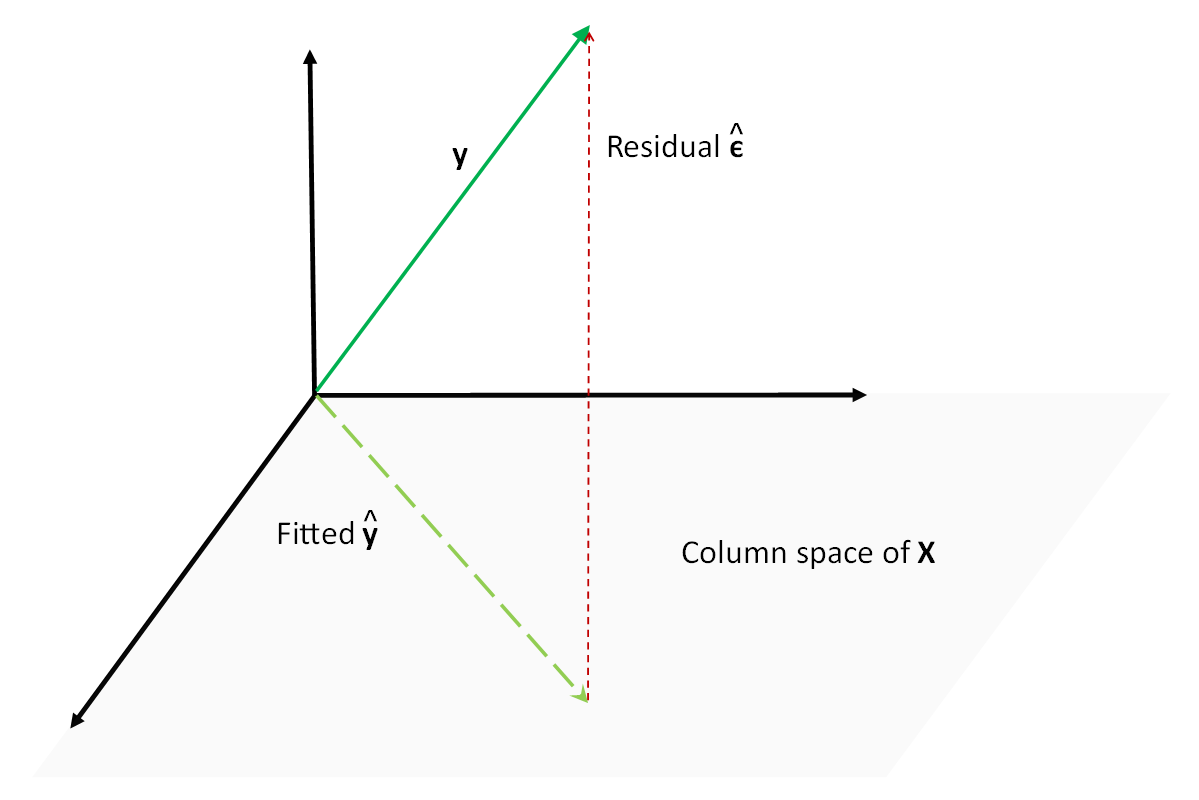
\includegraphics[scale=0.5]{0C__Users_tkpme_Dropbox_BookPCRA_Springer_Produ_____Stat_for_PCRM_Plots_OLS_Fit_Plus_Residual.png}
\par\end{centering}
\caption{OLS Orthogonal Projection and the Fit--plus--Residuals Decomposition}

\label{fig:OLSorthogonalProjectionGeometry}
\end{figure}

If $\mathbf{X}$ has full rank, i.e., if its columns are linearly
independent, then $\mathrm{\mathbf{X}}^{\prime}\,\mathrm{\mathbf{X}}$
is invertible, and the left hand side of \eqref{eq:OLSnormalEquations}
is easily rearranged to give
\begin{equation}
\hat{\bubeta}_{OLS}=\left(\mathrm{\mathbf{X}}^{\prime}\,\mathrm{\mathbf{X}}\right)^{-1}\,\mathrm{\mathbf{X}}^{\prime}\,\mathrm{\mathbf{y}},\label{eq:OLSbeta1}
\end{equation}
and the corresponding decomposition of $\mathrm{\mathbf{y}}$ into
the sum of its OLS fit plus a residual is

\begin{subequations}
\begin{align}
\hat{\mathrm{\mathbf{y}}} & =\mathbf{X}\ \hat{\bubeta}_{OLS}\label{eq:OLSFit}\\[0.5em]
\mathrm{\mathbf{y}} & =\hat{\mathbf{y}}\,+\,\hat{\bueps}.\label{eq:OLSFitPlusError}
\end{align}
\end{subequations}

If we subsitute \eqref{eq:OLSbeta1} into \eqref{eq:OLSFit}, we get

\begin{align}
\hat{\mathrm{\mathbf{y}}} & =\mathbf{X}\,\left(\mathrm{\mathbf{X}}^{\prime}\,\mathrm{\mathbf{X}}\right)^{-1}\,\mathrm{\mathbf{X}}^{\prime}\,\mathrm{\mathbf{y}}\nonumber \\
 & =\mathbf{H}\,\mathrm{\mathbf{y}},\label{eq:HatMatrix1}
\end{align}

where 

\begin{equation}
\mathbf{H}=\mathbf{X}\,\left(\mathrm{\mathbf{X}}^{\prime}\,\mathrm{\mathbf{X}}\right)^{-1}\,\mathrm{\mathbf{X}}^{\prime}\label{eq:HatMatrix2}
\end{equation}

is variously known as the \emph{Hat matrix} or the \emph{Projection}
\emph{matrix} as it projects $\mathbf{y}$ onto $\hat{\mathrm{\mathbf{y}}}$,
which lies in the column space of $\mathbf{X}$. The hat matrix is
symmetric and idempotent, i.e.

\begin{subequations}
\begin{align}
\mathbf{H}^{\prime} & =\mathbf{H}\label{eq:HatMatrix3}\\[0.5em]
\mathrm{\mathbf{H}} & =\mathrm{\mathbf{H}}^{2}.\label{eq:HatMatrix4}
\end{align}
\end{subequations}

It is easily seen that \eqref{eq:OLSFitPlusError} can be rewritten
using the Hat matrix as

\begin{align}
\hat{\bueps} & =\left(\mathbf{I}\,-\,\mathbf{H}\right)\mathbf{y}.\nonumber \\
 & =\mathbf{M}\,\mathbf{y},\label{eq:AnhillatorMatrix1}
\end{align}

where

\begin{equation}
\mathbf{M}=\mathbf{I}\,-\,\mathbf{H}\label{eq:AnhillatorMatrix2}
\end{equation}

is known as the \emph{Annihilator matrix}.

Even though \eqref{eq:LinearRegressionModel} is linear in $\mathbf{x}$,
it offers a powerful way in which to incorporate some, but not all,
of the nonlinearity in the relationship between the response variable
and the explanatory variables: for example, the columns of $\mathbf{X}$
can be non--linear transformations, and even cross--products that
capture possibly important interactions, of the individual explanatory
variables being used to predict $\mathrm{\mathbf{y}}$. In many cases
of practical interest, this simple modification significantly improves
the fit generated by \eqref{eq:OLSFit} \footnote{This technique is exploited in \ExpectedReturnChapter\  when forecasting
the returns of the S\&P 500 using its earnings and revenues.}, while taking advantage of the computational efficiency of a linear
model.

It is important to keep in mind that even though OLS is blessed with
an elegant theoretical foundation, it is not at all robust to outliers:
the OLS coefficients are linear in $\mathrm{\mathbf{y}}$, and consequently,
even a single outlier can make the bias in $\hat{\bubeta}_{OLS}$
arbitrarily large.\footnote{\citet{HeitmanOrd85} illuminate OLS's lack of robustness in a different
way -- they show that $\hat{\bubeta}_{OLS}$ is a weighted average
of all $\nicefrac{n!}{\left(m\,+\,1\right)!\left(n\,-\,m\,-\,1\right)!}$
possible coefficient vectors that can be formed using linear combinations
of $m\,+\,1$ rows of $\mathbf{X}$ and the corresponding rows of
$\mathrm{\mathbf{y}}$. A change to any single row induces a change
in each of the $\nicefrac{\left(n\,-\,1\right)!}{m!\left(n\,-\,m\,-\,1\right)!}$
coefficient vectors formed using it, making the weighted average not
robust to even a single outlier.} This greatly reduces its utility in fields such as finance where
data is plagued with outliers: OLS estimates can prove very misleading,
and it is for this reason that we stress the use of robust statistical
methods throughout this book.

\subsection{Weighted Least Squares}

Our development of OLS implicitly assumes that all observations are
equally important. But this is not necessarily true -- an investor
estimating the beta of a stock, for example, may be much more concerned
with its behavior in down markets than in up markets, or on days when
the market makes large moves. Equations \eqref{eq:OLSbeta} and \eqref{eq:OLSbeta1}
are easily modified to accommodate this requirement by overweighting
some observations and underweighting others.

Let $\mathrm{\mathbf{W}}$ be a diagonal \emph{weight matrix}, with
$\mathrm{\mathbf{W}}_{ii}\geqslant0$ being the weight assigned to
the $i^{th}$ observation. As $\mathrm{\mathbf{W}}$ is diagonal,
and as all of its entries are non--negative, it can be written as
a product

\begin{equation}
\mathrm{\mathbf{W}}=\mathrm{\mathbf{V}}^{\prime}\,\mathrm{\mathbf{V}},\label{eq:WeightMatrixAsProduct}
\end{equation}
where the diagonal entries of $\mathrm{\mathrm{\mathbf{V}}}$ and
$\mathrm{\mathbf{\mathbf{W}}}$ are related by
\begin{equation}
v_{i\,i}=\sqrt{w_{i\,i}},\ 1\leqslant i\leqslant n.\label{eq:VsquareRootW}
\end{equation}

To compute a down--market beta, for example, we set $v_{i\,i}=w_{i\,i}=0$
for all $i$ such that $r_{m,\,i}\geqslant0$ and $v_{i\,i}=w_{i\,i}=1$
for all $i$ such that $r_{m,\,i}<0$. The \emph{Weighted Least Squares}
(WLS) fit is the solution to
\begin{equation}
\hat{\bubeta}_{WLS}=\underset{\bubeta}{\mathrm{argmin}}\left(\mathrm{\mathbf{y}}\,-\,\mathrm{\mathbf{X}}\,\bubeta\right)^{\prime}\,\mathrm{\mathbf{W}}\,\left(\mathrm{\mathbf{y}}\,-\,\mathrm{\mathbf{X}}\,\bubeta\right).\label{eq:WLSbeta}
\end{equation}
The normal equations now become
\begin{align}
\mathbf{X}^{\prime}\,\mathbf{W}\,\left(\mathbf{y}\,-\,\mathbf{X}\,\hat{\bubeta}_{WLS}\right) & =\mathbf{X}^{\prime}\,\mathbf{W}\,\hat{\bueps}\nonumber \\
 & =\mathbf{0},\label{eq:WLSnormalEquations}
\end{align}
so that the residuals are orthogonal to the weighted regressors. Furthermore,
if $\mathbf{X}^{\prime}\,\mathbf{W}\,\mathbf{X}$ is invertible\footnote{This is equivalent to the condition that $\mathrm{\mathbf{X}}^{\prime}\,\mathrm{\mathbf{V}}$
has full rank.}, the left hand side of \eqref{eq:WLSnormalEquations} can be rearranged
to give
\begin{equation}
\hat{\bubeta}_{WLS}=\left(\mathrm{\mathbf{X}}^{\prime}\,\mathrm{\mathbf{W}}\,\mathrm{\mathbf{X}}\right)^{-1}\,\mathrm{\mathbf{X}}^{\prime}\,\mathrm{\mathbf{W}}\,\mathbf{y}.\label{eq:WLSbeta1}
\end{equation}
Equation \eqref{eq:WLSbeta} can be rewritten as

\begin{align}
\hat{\bubeta}_{WLS} & =\underset{\bubeta}{\mathrm{argmin}}\left(\mathbf{V}\,\left(\mathrm{\mathbf{y}}\,-\,\mathrm{\mathbf{X}}\,\bubeta\right)\right)^{\prime}\mathrm{\mathbf{\mathbf{V}}}\,\left(\mathrm{\mathbf{y}}\,-\,\mathrm{\mathbf{X}}\,\bubeta\right)\nonumber \\
 & =\underset{\bubeta}{\mathrm{argmin}}\left(\left(\mathbf{V}\,\mathrm{\mathbf{y}}\right)\,-\,\left(\mathbf{V}\,\mathrm{\mathbf{X}}\right)\,\bubeta\right)^{\prime}\,\left(\left(\mathbf{V}\,\mathrm{\mathbf{y}}\right)\,-\,\left(\mathbf{V}\,\mathrm{\mathbf{X}}\right)\,\bubeta\right).\label{eq:WLSBeta2}
\end{align}

Equation \eqref{eq:WLSBeta2} makes clear the fact that WLS is just
an application of OLS to a scaled set of response and predictor variables.
Alternatively, OLS can be viewed as a special case of \eqref{eq:WLSbeta}
in which $\mathrm{\mathbf{W}}=\mathrm{\mathbf{V}}=\mathrm{\mathbf{I}}_{n}$.

If the errors are heteroskedastic, i.e., if their variances are not
all the same, then the weights can be chosen to reflect the uncertainty
in the observations. A natural choice for the weights is $w_{ii}=\nicefrac{1}{\sigma_{i}^{2}}$,
where $\sigma_{i}^{2}$ is the known variance of $\epsilon_{i}$.
In fact, if the errors are uncorrelated and normally distributed with
mean 0, the WLS estimator with these weights is a maximum likelihood
estimator. This can be seen by letting $p_{0}$ in \eqref{eq: regMLEsknown}
be a standard normal distribution, replacing $s$ with $\sigma_{i}$,
and then carrying out the indicated minimization.

In most cases of interest, the error variances are not known in advance,
but must be estimated from the data, diminishing the benefits of WLS.
Even so, the WLS estimate often represents a significant improvement
over its OLS counterpart. Robust regression methods, in particular,
are at heart specialized variants of WLS that automate the process
of identifying and underweighting outliers using data dependent weights,
which greatly diminishes their impact on the solution to \eqref{eq:WLSbeta}.
It is shown in \RobustMethodsChapters\ that data dependent weights
can be represented as
\begin{equation}
w_{ii}=\frac{\psi\left(\hat{\epsilon}_{i}\right)}{\hat{\epsilon}_{i}},\label{eq:RobustRegressionW}
\end{equation}
where $\psi\left(.\right)$ is a nonlinear transformation that is
applied to the residuals, and which systematically underweights outliers.

\subsection{Generalized Least Squares}

\emph{Generalized Least Squares} (GLS) combines two important ideas
to identify an optimal set of coefficients for the linear regression
model when its errors are correlated.
\begin{enumerate}
\item Individual observations can be weighted in inverse proportion to the
variance of their residuals to equalize their relative importance
(the same idea was earlier applied in our discussion of Weighted Least
Squares), and
\item The distance between a vector of correlated residuals and the mean
of their joint distribution can be computed using a scale invariant
distance measure known as the \emph{Mahalanobis distance}.\footnote{See Appendix A for a discussion of the Mahalanobis distance.}
\end{enumerate}
Formally, the GLS fit is the solution to
\begin{equation}
\hat{\bubeta}_{GLS}=\underset{\bubeta}{\mathrm{argmin}}\left(\mathrm{\mathbf{y}}\,-\,\mathrm{\mathbf{X}}\,\bubeta\right)^{\prime}\,\mathrm{\mathbf{C}^{-1}}\,\left(\mathrm{\mathbf{y}}\,-\,\mathrm{\mathbf{X}}\,\bubeta\right),\label{eq:GLSbeta}
\end{equation}
where $\mathbf{C}$ is the known, non--singular, covariance matrix
of the errors. Replacing our diagonal weight matrix $\mathrm{\mathbf{W}}$
with $\mathbf{C}^{-1}$ simultaneously scales and decorrelates the
errors, and equalizes the relative importance of each term in \eqref{eq:GLSbeta}.

If $\mathrm{\mathbf{X}}^{\prime}\,\mathrm{\mathbf{C}^{-1}}\,\mathrm{\mathbf{X}}$
is invertible, the GLS coefficients are
\begin{equation}
\hat{\bubeta}_{GLS}=\left(\mathrm{\mathbf{X}}^{\prime}\,\mathrm{\mathbf{C}^{-1}\,}\mathrm{\mathbf{X}}\right)^{-1}\,\mathrm{\mathbf{X}}^{\prime}\,\mathbf{C}^{-1}\,\mathrm{\mathbf{y}}.\label{eq:GLSbeta1}
\end{equation}
As $\mathbf{C}^{-1}$ is square, symmetric, and positive definite,
it can be factored as\footnote{See the discussion of the Singular Value Decomposition in Appendix
A,}
\begin{equation}
\mathbf{C}^{-1}=\buOmega^{\prime}\,\buOmega,\label{eq:CinverseDecomposition}
\end{equation}
and we can rewrite \eqref{eq:GLSbeta} as
\begin{align}
\hat{\bubeta}_{GLS} & =\underset{\bubeta}{\mathrm{argmin}}\left(\left(\mathbf{\buOmega\,}\mathrm{\mathbf{y}}\right)\,-\,\left(\mathbf{\buOmega\,}\mathrm{\mathbf{X}}\right)\,\bubeta\right)^{\prime}\,\left(\left(\mathbf{\buOmega}\,\mathrm{\mathbf{y}}\right)-\left(\mathbf{\buOmega}\,\mathrm{\mathbf{X}}\right)\,\bubeta\right),\label{eq:GLSBeta2}
\end{align}
illuminating the fact that GLS is just the application of OLS to a
particular transformation of the raw data\footnote{See Chapter 1 of \citet{Hayashi2000} or Chapter 9 of \citet{Greene2018}
for a lucid description of GLS and its properties.}.

Unfortunately, $\hat{\bubeta}_{GLS}$, like $\hat{\bubeta}_{OLS}$,
is linear in $\mathrm{\mathbf{y}}$, and GLS therefore inherits OLS's
primary failing -- it is not robust to the presence of even a single
outlier. In addition, $\mathrm{\mathbf{C}}$ is usually not known,
and must be estimated from data. The estimation process is inherently
noisy, and widens the distribution of $\hat{\bubeta}_{GLS}$, eroding
much of the theoretical advantage of GLS over WLS and OLS. Furthermore,
the finite sample properties of the GLS estimator with an unknown
covariance matrix are not known, and as a consequence, OLS and WLS
see far more use in practice than does GLS. 

\subsection{Least Squares Inference with Normally Distributed Errors}

In some special cases, OLS yields information about the distribution
of the regression coefficients, allowing us to test hypotheses about
their value. In particular, if the errors have an i.i.d. normal distribution,
i.e., if
\begin{equation}
\bueps\,|\,\mathrm{\mathbf{X}}\,\sim\,\mathrm{MVN}\left(0,\ \sigma^{2}\,\mathrm{\mathbf{I}}_{n}\right)\ \forall\,\mathbf{X},\label{eq:MultivariateNormalErrors}
\end{equation}
the sampling distribution of the regression coefficients is also multivariate
normal, as
\begin{align}
\hat{\bubeta}_{OLS}\,\mathrm{-\,}\bubeta & =\left(\mathrm{\mathbf{X}}^{\prime}\,\mathrm{\mathbf{X}}\right)^{-1}\,\mathrm{\mathbf{X}}^{\prime}\,\mathrm{\mathbf{y}}\,\mathrm{-\,}\bubeta\nonumber \\
 & =\left(\mathrm{\mathbf{X}}^{\prime}\,\mathrm{\mathbf{X}}\right)^{-1}\,\mathrm{\mathbf{X}}^{\prime}\,\left(\mathrm{\mathbf{X}}\,\bubeta\,+\,\bueps\right)\,\mathrm{-\,}\bubeta\nonumber \\
 & =\left(\mathrm{\mathbf{X}}^{\prime}\,\mathrm{\mathbf{X}}\right)^{-1}\,\mathrm{\mathbf{X}}^{\prime}\,\bueps.\label{eq:BetaRelatesToEpsilon}
\end{align}

It follows that the covariance matrix of the sampling errors of the
regression coefficients is given by
\begin{equation}
Cov\left(\hat{\bubeta}_{OLS}\,|\,\mathrm{\mathbf{X}}\right)\sim\mathrm{MVN}\left(0,\ \sigma^{2}\,\left(\mathrm{\mathbf{X}}^{\prime}\,\mathrm{\mathbf{X}}\right)^{-1}\right).\label{eq:MultivariateNormalSamplingErrors}
\end{equation}
Even though $\sigma^{2}$ is unknown, we can obtain an unbiased estimate
of it using the squared residuals \footnote{The denominator of \eqref{eq:sSquared} is $n\,-\,m\,-\,1$, and not
$n\,-\,m$, because we have a total of $m\,+\,1$ explanatory variables:
an intercept and $m$ predictor variables. In some textbooks, $x_{1}$
is assumed to be the intercept, which reduces the number of explanatory
variables to $m$ and makes the denominator $n\,-\,m$.}

\begin{equation}
s^{2}=\frac{\hat{\bueps}^{\prime}\ \hat{\bueps}}{n\,-\,m\,-\,1},\label{eq:sSquared}
\end{equation}
using which the standard error of the $j^{th}$ regression coefficient
can be computed as:

\begin{equation}
SE\left(\hat{\beta}_{j,\,OLS}\right)=\sqrt{s^{2}\,\times\,\left(\left(\mathrm{\mathbf{X}}^{\prime}\,\mathrm{\mathbf{X}}\right)^{-1}\right)_{j,\,j}}\,,\ 1\leqslant j\leqslant m+1.\label{eq:SEofBetaj}
\end{equation}

If we have a hypothesized value for $\beta_{j}$, say $\overline{\beta_{j}}$,
we can test the hypothesis
\begin{equation}
H_{0}:\ \beta_{j}=\overline{\beta_{j}}\label{eq:NullHypothesis}
\end{equation}
using the t--test, whose t--statistic
\begin{equation}
t_{j}=\frac{\hat{\beta}_{j,\,OLS}\,-\,\overline{\beta_{j}}}{SE\left(\hat{\beta}_{j,\,OLS}\right)},\label{eq:tStatRegression}
\end{equation}
has a $t$ distribution with $n\,-\,m\,-\,1$ degrees of freedom.

If we specify a two--sided significance level $\alpha$, we can reject
the null hypothesis if the $t$--statistic is sufficiently large,
i.e., if
\begin{equation}
|t_{j}|>t_{\alpha/2}\left(n\,-\,m\,-\,1\right).\label{eq:tTestRegression}
\end{equation}

Often, $\overline{\beta_{j}}$ is set to 0, so that the null hypothesis
corresponds to $x_{j}$ being unrelated to $y$ and thus superfluous
to the model, and its rejection corresponds to the identification
of a useful explanatory variable. The $t$--test finds use with non--zero
values of $\overline{\beta_{j}}$ as well: for example, when testing
the validity of the single--factor CAPM model for a young, fast--growing
firm with a volatile stock, the null hypothesis might reflect our
belief that its true beta is 2, and this hypothesis can be tested
by running a regression followed by a $t$--test.

More generally, we can use the $F$ test to test the linear hypothesis
\begin{equation}
H_{0}:\ \mathrm{\mathbf{A}}\bubeta=\mathrm{\mathbf{a}},\label{eq:FTest1}
\end{equation}
where $\mathrm{\mathbf{a}}$ is an $p\,\times\,1$ vector, and $\mathrm{\mathbf{A}}$
is a $p\,\times\,\left(m\,+\,1\right)$ matrix with rank $p$. Common
uses of this specification include testing the hypothesis that two
or more of the coefficients are simultaneously equal to pre--specified
values (often 0), or that their sum or difference is equal to a constant.
In fact, \eqref{eq:NullHypothesis} can be viewed as a special case
of \eqref{eq:FTest1} in which $\mathrm{\mathbf{a}}=0$ and $\mathbf{A}$
is a $1\,\times\,\left(m\,+\,1\right)$ matrix with 1 in its $j\,+\,1^{st}$
column and 0's elsewhere.

It is shown in Proposition 1.4 of \citet{Hayashi2000} that under
the null hypothesis \eqref{eq:FTest1}, the $F$ statistic
\begin{equation}
F=\frac{\left(\mathrm{\mathbf{A}}\,\hat{\bubeta}_{OLS}\,-\,\mathrm{\mathbf{a}}\right)^{\prime}\left(\mathrm{\mathbf{A}}\left(\mathrm{\mathbf{X}}^{\prime}\,\mathrm{\mathbf{X}}\right)^{-1}\mathrm{\mathbf{A}}^{\prime}\right)^{-1}\left(\mathrm{\mathbf{A}}\,\hat{\bubeta}_{OLS}\,-\,\mathrm{\mathbf{a}}\right)}{p\cdot s^{2}}\label{eq:Fstatistic}
\end{equation}
with $s^{2}$ defined in \eqref{eq:sSquared}, has a $F\left(p,\ n\,-\,m\,-\,1\right)$
distribution with $p$ degrees of freedom in the numerator and $n\,-\,m\,-\,1$
degrees of freedom in the denominator.

The null hypothesis is rejected at significance level $\alpha$ if
\begin{equation}
F>F_{\alpha}\left(p,\ n\,-\,m\,-\,1\right),\label{eq:FTestRegression}
\end{equation}
where $F_{\alpha}\left(.\right)$ is the critical value of the $F$
distribution corresponding to a tail probability of $\alpha$. The
$t$ and $F$ distributions are related: it can be shown that if a
random variable $u$ has a $t(q)$ distribution, $u^{2}$ has an $F\left(1,\ q\right)$
distribution.

The $F$ test can be extended to cover both WLS and GLS, and \citet{ScarianoDavenport1984}
derive an exact expression for the \emph{Corrected F--statistic,
$F^{W}$}. They show that $F^{W}$ has a non--central $F$ distribution
with parameters $p,\ n\,-\,m\,-\,1$ and $\lambda$, where $\lambda$
is a complex function of $\mathrm{\mathbf{A},\ }\hat{\bubeta}_{GLS},\ \mathrm{\mathbf{a},}\ \mathbf{X,\ \mathrm{\mathbf{y}}}$
and $\mathrm{\mathbf{C}}$, the known covariance matrix of the errors.
We refer the interested reader to \citet{ScarianoDavenport1984} for
the relevant formulae.

In spite of the elegance of these results, great care must be taken
with their application. The conditions under which they hold are rarely
satisfied in practice, and \eqref{eq:tTestRegression} and \eqref{eq:FTestRegression}
often lead to erroneous judgments concerning the significance of explanatory
variables. \citet{Harvey2017}, \citet{Harvey2019}, and \citet{BRR2021}
illuminate the ease with which such errors of judgment arise when
running batteries of tests against financial data, and describe enhancements
to \eqref{eq:tTestRegression} and \eqref{eq:FTestRegression} that
usefully protect against false findings of significance\footnote{A variety of techniques for correcting some of the effects of multiple
testing, endogeneity and overlapping observations are described and
used in \ExpectedReturnChapter. Unfortunately, they are not exhaustive
-- in many settings, there is no credible way in which to correct
for the collective impact of these distortions, and we are forced
to use simulations to approximate the distribution of parameters under
the null hypothesis. Approximate critical values for each significance
level can be obtained from the simulation, and the estimated parameter
can be compared to the approximate critical values to obtain an approximate
significance level.}.

\subsection{The Gauss--Markov Theorem\label{subsec:GaussMarkovTheorem}}

Under the following four assumptions:
\begin{enumerate}
\item The relationship between $\mathrm{\mathbf{y}}$ and $\mathrm{\mathbf{X}}$
is described by the linear regression model: $\mathrm{\mathbf{y}}=\mathrm{\mathbf{X}}\,\bubeta\,+\,\bueps$,\footnote{Most introductory textbooks on linear regression assume that $\mathrm{\mathbf{X}}$
is fixed and non--random, but for applications in finance and economics,
the columns of $\mathrm{\mathbf{X}}$ should be thought of as a collection
of of random vectors.}
\item The error term satisfies $\mathrm{E}\left(\bueps\,|\,\mathrm{\mathbf{X}}\right)=\mathbf{0}$.
In econometrics textbooks, this condition is referred to as \emph{strict
exogeneity},
\item Lack of collinearity: the rank of the data matrix is equal to $m+1$,
the number of columns it contains, with probability 1, and
\item The  errors are conditionally uncorrelated and their conditional
variances are identical: $\mathrm{E}\left(\bueps\,\bueps^{\prime}\,|\,\mathrm{\mathbf{X}}\right)=\sigma^{2}\,\mathrm{\mathbf{I}}_{n}$,
\end{enumerate}
the celebrated \emph{Gauss--Markov theorem}\footnote{See Chapter 1 of \citet{Hayashi2000} or Chapter 4 of \citet{Greene2018}
for a proof of the Gauss--Markov theorem.} states that the OLS estimator is the \emph{best linear unbiased estimator}
(BLUE) in the sense that $\mathbf{\Sigma}_{\hat{\bubeta}_{OLS}}$,
the covariance matrix of its coefficient estimates, is not larger
than \footnote{An $n\times n$ matrix $\mathrm{\mathbf{A}}_{1}$ is said to be smaller
than another $n\times n$ matrix $\mathrm{\mathbf{A}}_{2}$ if the
difference of the two matrices, $\Delta\mathrm{\mathbf{A}}=\mathrm{\mathbf{A}}_{2}-\mathrm{\mathbf{A}}_{1}$,
is positive definite,} the covariance matrix of the coefficients of any other unbiased linear
estimator. If we additionally assume that the errors are normally
distributed, the OLS estimates are actually maximum likelihood estimates
(see Section \ref{subsec:RegressionModelMLEs} for details), though
this is a very stringent requirement that is hardly ever satisfied
in practice.

As GLS can be viewed as an application of OLS to a set of transformed
variables, it inherits the virtues of OLS: it is equivalent to the
maximum likelihood estimator for normally distributed errors, satisfies
the Gauss--Markov theorem when Assumption 4 is changed to restrict
the conditional covariance matrix of the errors only to be positive
definite, and is BLUE. Additionally, $\hat{\bubeta}_{GLS}$ is unbiased
and consistent\footnote{\citet{Hansen2021} generalizes the Gauss--Markov theorem and shows
that the OLS and GLS estimators are actually the best unbiased estimators
of the regression coefficients (BUE), and that there is no need to
restrict attention to the class of linear estimators. In fact, he
shows that any estimator of the regression coefficients which has
a smaller covariance matrix must necessarily be biased. The qualification
that the estimator be unbiased is important -- it has long been known
that some estimators, such as the \citet{JamesStein1961} estimator,
allow a small increase in bias in return for a much larger decrease
in variance. That said, unbiased estimators continue to play a central
role in estimation, as they are far more easily analyzed than their
biased counterparts.}. But, as we have earlier noted, GLS also inherits OLS's greatest
liability -- its lack of robustness to outliers \footnote{\citet{EfronMorris1973} explore Stein's estimator in an Empirical
Bayes setting, and \citet{EfronMorris1977} provide a very readable
account of the estimator and its associated paradox, and apply it
to baseball scores in the 1970 season as well as to the incidence
of toxoplasmosis in El Salvador.}. 

\section{Minimum Mean Squared Error (MMSE) Predictors\label{sec:MMSEPredictors}}


\subsection{MMSE Predictors of a Scalar Random Variable\label{subsec:MMSEPredictors}}

We earlier assumed that $\mathrm{\mathbf{x}}$ and $\mathrm{\mathbf{y}}$
were vectors whose entries were drawn from an unknown distribution,
but we now assume that they are drawn from some known joint distribution.
For simplicity, we start by considering a scalar random variable $y$
whose value we wish to predict using a vector of predictors $\mathrm{\mathbf{x}}$.
In general, a predictor for $y$ based on $\mathrm{\mathbf{x}}$ can
be written as
\begin{equation}
\hat{y}=g\left(\mathrm{\mathbf{x}}\right),\label{eq:MMSEscalar1}
\end{equation}
where $\hat{y}$ is the predicted value of $y$, and $g\left(\cdotp\right)$
is an arbitrary function. In many cases of practical interest in finance,
$y$ can be observed only in the future, while the components of $\mathrm{\mathbf{x}}$
are observed at the present time, so that \eqref{eq:MMSEscalar1}
is often best thought of as
\begin{equation}
\hat{y}_{t\,+\,1}=g\left(\mathrm{\mathbf{x}}_{t}\right).\label{eq:MMSEscalar2}
\end{equation}

Once $y$ has been observed, we can compute the prediction error
\begin{equation}
e=y\,-\,\hat{y},\label{eq:PredictionError}
\end{equation}
where $y$, with some abuse of notation, denotes the realization of
the random variable in \eqref{eq:PredictionError}.\footnote{It is the norm in most probability textbooks to use capital letters
for random variables and small letters for their realizations. This
textbook, however, has random variables, random vectors and random
matrices, as well as their realizations, to represent, and consistency
in one place often opens up an inconsistency in another, or necessitates
the use of obscure and clumsy notation. We therefore take the liberty
of using the same letter to denote both the random variable and its
realization, and where needed for clarity to distinguish a random
variable from its realized value, we will do so in a footnote.

} The \emph{mean squared prediction error} conditioned on a particular
value of $\mathrm{\mathbf{x}}$ is
\begin{align}
{\mathrm{MSE}}_{\mathrm{\mathbf{x}}} & =\mathrm{E}_{y}\left[e^{2}\,|\,\mathrm{\mathbf{x}}\right]\nonumber \\
 & =\mathrm{E}_{y}\left[\left(y\,-\,\hat{y}\right)^{2}\,|\,\mathrm{\mathbf{x}}\right]\nonumber \\
 & =\mathrm{E}_{y}\left[\left(y\,-\,g\left(\mathrm{\mathbf{x}}\right)\right)^{2}\,|\,\mathrm{\mathbf{x}}\right],\label{eq:MSE}
\end{align}
and the \emph{Minimum Mean Squared Error} \emph{Predictor}, $g_{0}\left(\mathrm{\mathbf{x}}\right)$,
which minimizes \eqref{eq:MSE}, is given by
\begin{equation}
g_{0}\left(\mathrm{\mathbf{x}}\right)=\mathrm{E}_{y}\left[y\,|\,\mathrm{\mathbf{x}}\right],\label{eq:MMSEPredictor}
\end{equation}
where $\mathrm{E}_{y}\left[y\,|\,\mathrm{\mathbf{x}}\right]$ is the
conditional mean of the random variable $y$ conditioned on $\mathrm{\mathbf{x}}$.
This can be seen by writing
\begin{equation}
\mathrm{E}_{y}\left[\left(y\,-\,g\left(\mathrm{\mathbf{x}}\right)\right)^{2}\,|\,\mathrm{\mathbf{x}}\right]=\intop\left(y\,-\,g\left(\mathrm{\mathbf{x}}\right)\right)^{2}f_{y\,|\,\mathrm{\mathbf{x}}}\,dy\label{eq:MMSEIntegral}
\end{equation}
where $f_{y\,|\,\mathrm{\mathbf{x}}}$ is the conditional density
of $y$. If we differentiate \eqref{eq:MMSEIntegral} with respect
to $g\left(\mathrm{\mathbf{x}}\right)$\footnote{For any fixed value of $\mathrm{\mathbf{x}}$, $g\left(\mathrm{\mathbf{x}}\right)$
is a scalar, and can be thought of as a parameter with respect to
which the integral is differentiated.} and set the resulting expression to 0, we get
\begin{equation}
2\intop\left(g_{0}\left(\mathrm{\mathbf{x}}\right)\,-\,y\right)f_{y\,|\,\mathrm{\mathbf{x}}}\,dy=0.\label{eq:MMSEDerivativeEq0}
\end{equation}

The first term in \eqref{eq:MMSEDerivativeEq0} equals $g_{0}\left(\mathrm{\mathbf{x}}\right),$and
it follows that
\begin{align}
g_{0}\left(\mathrm{\mathbf{x}}\right) & =\intop y\,f_{y\,|\,\mathrm{\mathbf{x}}}\,dy\nonumber \\
 & =\mathrm{E}_{y}\left[y\,|\,\mathrm{\mathbf{x}}\right].\label{eq:MMSEProof}
\end{align}
Differentiating \eqref{eq:MMSEDerivativeEq0} a second time makes
clear that the second derivative is strictly positive so that \eqref{eq:MMSEProof}
represents a minimum, and not a stationary point. Since the conditional
mean predictor $g_{0}\left(\mathrm{\mathbf{x}}\right)$ minimizes
the conditional MSE for every $\mathbf{x}$, it must also minimize
the unconditional MSE. To see that this is true, observe that the
unconditional MSE of the predictor is  
\begin{align}
\mathrm{E}_{\mathbf{x}}\left[{\mathrm{MSE}}_{\mathrm{\mathbf{x}}}\right] & =\mathrm{E}_{\mathbf{x}}\left[\mathrm{E}_{y}\left[\left(y\,-\,g_{0}\left(\mathrm{\mathbf{x}}\right)\right)^{2}\,|\,\mathrm{\mathbf{x}}\right]\right]\nonumber \\
 & =\idotsint\left(y\,-\,g_{0}\left(\mathrm{\mathbf{x}}\right)\right)^{2}\,f_{y,\,\mathrm{\mathbf{x}}}\,dy\,d\mathbf{x}.\label{eq:UnconditionalMSE}
\end{align}
But $f_{y,\,\mathrm{\mathbf{x}}}$ is non-negative, and it follows
that minimizing \eqref{eq:MMSEIntegral} for each value of $\mathrm{\mathbf{x}}$
simultaneously minimizes \eqref{eq:UnconditionalMSE}. While we could,
in principle, have started with the objective of minimizing the unconditional
MSE, the path we have chosen greatly enhances the clarity of the exposition
of this important result.

The MMSE predictor is unbiased in that the expected value of its prediction
is identical to the expected value of the random variable $y$. The
notion of unbiasedness presented in subsection \ref{subsec: estUnbiased},
in contrast, is concerned with bias in the estimation of an unknown,
but constant, parameter.

Remarkably, the prediction error of the MMSE predictor is orthogonal
to \emph{any} function of $\mathbf{x}$, i.e.
\begin{align}
\mathrm{E}_{\,y,\,\mathrm{\mathbf{x}}}\left[\left(y\,-\,g_{0}\left(\mathrm{\mathbf{x}}\right)\right)h\left(\mathbf{x}\right)\right] & =\mathrm{E}_{\mathrm{\mathbf{x}}}\left[E_{\,y\,|\,\mathrm{\mathbf{x}}}\left[\left(y\,-\,g_{0}\left(\mathrm{\mathbf{x}}\right)\right)h\left(\mathbf{x}\right)\thinspace|\,\mathrm{\mathbf{x}}\right]\right]\nonumber \\
 & =\mathrm{E}_{\mathrm{\mathbf{x}}}\left[\left(\mathrm{E}_{\,y\,|\,\mathrm{\mathbf{x}}}\left[y\right]\,-\,\mathrm{E}\left[y\,|\,\mathrm{\mathbf{x}}\right]\right)h\left(\mathbf{x}\right)\thinspace|\,\mathrm{\mathbf{x}}\right]\nonumber \\
 & =\mathrm{E}_{\mathrm{\mathbf{x}}}\left[\left(\mathrm{E}\left[y\,|\,\mathrm{\mathbf{x}}\right]\,-\,\mathrm{E}\left[y\,|\,\mathrm{\mathbf{x}}\right]\right)h\left(\mathbf{x}\right)\thinspace|\,\mathrm{\mathbf{x}}\right]\nonumber \\
 & \mathrm{=0}.\label{eq:OrthogonalityPrinciple}
\end{align}


\subsection{Linear MMSE Predictors of a Scalar Random Variable\label{subsec:LinearMMSEScalar}}

Even though \eqref{eq:MMSEPredictor} is true in general, it is not
always easy to implement -- $f_{y\,|\,\mathrm{\mathbf{x}}}$ is not
usually known, and even if it is, it may be non--linear, time--varying,
and computationally taxing. A widely used solution to these problems
is to restrict $g\left(\mathrm{\mathbf{x}}\right)$ to be an affine
function of $\mathrm{\mathbf{x}}$, and to write
\begin{equation}
\hat{y}=\alpha\,+\,\mathrm{\mathbf{x}}^{\prime}\,\bubeta\label{eq:LinearMMSEAppB1}
\end{equation}
where $\alpha$ is a constant, $\mathbf{x}$ is the known observable
and $\bubeta$\ is a vector of unknown coefficients\footnote{For clarity of exposition, $\bubeta$ reflects only the weights applied
to the random variables -- the constant $\alpha$ is treated separately.
In our earlier development of OLS, in contrast, our problem formulation
was greatly simplified by making $\alpha$ the first entry in $\bubeta$.}.

As in our earlier development of OLS, even though \eqref{eq:LinearMMSEAppB1}
is affine in $\mathbf{x}$, we can incorporate some, but not all,
of the nonlinearity that \eqref{eq:MMSEscalar1} admits: the elements
of $\mathbf{x}$ can be non--linear transformations, and even cross--products,
of the raw data being used to forecast $y$. In many cases of practical
interest, this simple modification significantly lowers the mean squared
prediction error of the forecasts generated by \eqref{eq:LinearMMSEAppB1}.

In the special case when $\mathrm{\mathbf{x}}$ is jointly normally
(or more generally, jointly elliptically) distributed with a finite
variance, $\mathrm{E}\left(y\,|\,\mathrm{\mathbf{x}}\right)$ is given
exactly by \eqref{eq:LinearMMSEAppB1}\footnote{See \citet{CambanisHuangSimons1981} and \citet{Ding2016} for a proof.},
but this is not very useful for asset returns because of their known
non--normality\footnote{\citet{AzzaliniCapitanio2014} is a useful reference for non--normal
and skewed distributions.}. Instead, by minimizing
\begin{equation}
\mathrm{E}\left[\left(y\,-\,\alpha\,-\,\mathrm{\mathbf{x}}^{\prime}\,\bubeta\right)^{2}\right],\label{eq:LinearMMSEAppB2}
\end{equation}
we show in subsection \ref{subsec:OptimalityLMMSE} that the linear
MMSE predictor of $y$ is obtained by setting

\begin{subequations}
\begin{align}
\bubeta_{LMMSE} & =\mathrm{\mathbf{C}}^{-1}\,\busigma\label{eq:LinearMMSEbetaAppB}\\[0.5em]
\alpha_{LMMSE} & =\mathrm{E}\left[y\right]\,-\,\mathrm{E\left[\mathbf{x}\right]}^{\prime}\,\bubeta_{LMMSE},\label{eq:LinearMMSEalphaAppB}
\end{align}
\end{subequations}

where $\mathbf{C}$ is the covariance matrix of $\mathbf{x}$ and
$\busigma=\mathrm{cov}\left(y,\,\mathbf{x}\right)$.

In the special case when $\mathbf{x}$ is a scalar, denoted by $x$,
\begin{equation}
\hat{y}=\mathrm{E}\left[y\right]\,+\,\frac{\mathrm{cov}\left(x,\,y\right)}{\sigma_{x}^{2}}\left(x\,-\,\mathrm{E}\left[x\right]\right).\label{eq:LinearMMSEAppB4}
\end{equation}
The minimum mean squared error of the Linear MMSE predictor is
\begin{align}
\mathrm{MMSE} & =\sigma_{y}^{2}\,-\,\busigma^{\prime}\,\mathrm{\mathbf{C}}^{-1}\,\busigma\nonumber \\
 & =\sigma_{y}^{2}\left(1\,-\,R_{y,\,\mathbf{x}}^{2}\right),\label{eq:LinearMMSEAppB3}
\end{align}
where
\begin{equation}
R_{y,\,\mathbf{x}}^{2}=\frac{\busigma^{\prime}\,\mathrm{\mathbf{C}}^{-1}\,\busigma}{\sigma_{y}^{2}}\label{eq:RsquaredYx}
\end{equation}
is the fraction of the variance of $y$ explained by $\mathbf{x}$.

The LMMSE predictor is clearly unbiased. That said, it is important
to keep in mind that  $\alpha$, $\bubeta$ and $\mathrm{\mathbf{C}}$
are usually not known, but must be estimated from data. While a rich
body of work on optimal estimators exists for data drawn from known
distributions, most classical estimators are sensitive to misspecification
and to outliers, necessitating the use of robust estimators such as
\texttt{lmrobdetMM} and \texttt{covRob} in the R package \texttt{RobStatTM}
for many problems in finance and economics.

\subsection{Optimality and MSE of the LMMSE Predictor\label{subsec:OptimalityLMMSE}}

To prove the optimality of the LMMSE predictor, we follow much the
same sequence of steps we used in \ref{subsec:MMSEPredictors}. The
prediction error is now given by
\begin{align*}
e & =y\,-\,\alpha\,-\,\mathrm{\mathbf{x}}^{\prime}\bubeta.
\end{align*}
and the \emph{unconditional}\footnote{We focus on the unconditional MSE because we want $\alpha$ and $\bubeta$
to be fixed constants that, unlike $\mathrm{E}\left(y\,|\,\mathbf{x}\right)$,
do not depend on the realization of $\mathbf{x}$.} mean squared prediction error becomes
\begin{align}
\mathrm{MSE} & =\mathrm{E}_{y,\mathbf{x}}\left[\left(y\,-\,\alpha\,-\,\mathrm{\mathbf{x}}^{\prime}\bubeta\right)^{2}\right]\nonumber \\
 & =\idotsint\left(y\,-\,\alpha\,-\,\mathrm{\mathbf{x}}^{\prime}\bubeta\right)^{2}\,f_{y,\,\mathrm{\mathbf{x}}}\,dy\,d\mathbf{x}.\label{eq:LMMSE1}
\end{align}

Differentiating \eqref{eq:LMMSE1} with respect to $\alpha$, evaluating
the integrals, and set the resulting expression to 0 gives
\begin{align}
\alpha= & \mathrm{E}\left[y\right]\,-\,\mathrm{E}\left[\mathrm{\mathbf{x}}\right]^{\prime}\,\bubeta.\label{eq:ExpectedYgivenX}
\end{align}
To obtain $\bubeta$, we substitute \eqref{eq:ExpectedYgivenX} into
\eqref{eq:LMMSE1} to get
\begin{align}
\mathrm{MSE} & =\idotsint\left(\left(y\,-\,\mathrm{E}\left[y\right]\right)\,-\,\left(\mathrm{\mathbf{x}}\,-\,\mathrm{E}\left[\mathrm{\mathbf{x}}\right]\right)^{\prime}\bubeta\right)^{2}f_{y,\,\mathrm{\mathbf{x}}}dyd\mathbf{x}.\nonumber \\
 & =\idotsint\left(\left(y\,-\,\mathrm{E}\left[y\right]\right)^{2}\,-\,2\left(y\,-\,\mathrm{E}\left[y\right]\right)\left(\mathrm{\mathbf{x}}\,-\,\mathrm{E}\left[\mathrm{\mathbf{x}}\right]\right)^{\prime}\,\bubeta\,+\,\bubeta^{\prime}\,\left(\mathrm{\mathbf{x}}\,-\,\mathrm{E}\left[\mathrm{\mathbf{x}}\right]\right)\left(\mathrm{\mathbf{x}}\,-\,\mathrm{E}\left[\mathrm{\mathbf{x}}\right]\right)^{\prime}\,\bubeta\right)\,f_{y,\mathrm{\,\mathbf{x}}}dyd\mathbf{x}\nonumber \\
 & =\sigma_{y}^{2}\,-\,2\,\busigma^{\prime}\,\bubeta\,+\,\bubeta^{\prime}\,\mathrm{\mathbf{C}}\,\bubeta\label{eq:LMMSE2}
\end{align}
where $\busigma$ and $\mathrm{\mathbf{C}}$ are defined immediately
below \eqref{eq:LinearMMSEbetaAppB} and \eqref{eq:LinearMMSEalphaAppB}.

The gradient of \eqref{eq:LMMSE2}, which must be $\boldsymbol{0}$
when MSE is minimized, is
\begin{align}
\nabla\left(\sigma_{y}^{2}\,-\,2\busigma^{\prime}\,\bubeta\,+\,\bubeta^{\prime}\,\mathrm{\mathbf{C}}\,\bubeta\right) & =-2\,\busigma\,+\,2\,\mathrm{\mathbf{C}}\,\bubeta.\label{eq:LMMSE3}
\end{align}
Additionally, the Hessian of the MSE is
\begin{align}
\mathrm{\mathbf{H}}\left(\sigma_{y}^{2}\,-\,2\busigma^{\prime}\,\bubeta\,+\,\bubeta^{\prime}\,\mathrm{\mathbf{C}}\,\bubeta\right) & =2\,\mathrm{\mathbf{C}}.\label{eq:LMMSE3a}
\end{align}
which is positive definite, implying that the stationary point is
a minimum, and that
\begin{equation}
\busigma=\mathrm{\mathbf{C}}\,\bubeta\label{eq:LMMSE4}
\end{equation}
and
\begin{equation}
\bubeta=\mathrm{\mathbf{C}^{-1}}\,\busigma.\label{eq:LMMSE5}
\end{equation}
It follows that 
\begin{align}
\mathrm{MSE} & =\sigma_{y}^{2}\,-\,\bubeta^{\prime}\,\mathrm{\mathbf{C}}\,\bubeta\nonumber \\
 & =\sigma_{y}^{2}\,-\,\busigma^{\prime}\,\mathrm{\mathbf{C}^{-1}}\,\busigma.\label{eq:LMMSE6}
\end{align}

The second term on the right hand side of \eqref{eq:LMMSE6} can be
further simplified using \eqref{eq:LMMSE4} and \eqref{eq:LMMSE5}
\begin{align}
\busigma^{\prime}\,\mathrm{\mathbf{C}^{-1}}\,\busigma & =\frac{\left(\busigma^{\prime}\,\mathrm{\mathbf{C}^{-1}}\,\busigma\right)^{2}}{\busigma^{\prime}\,\mathrm{\mathbf{C}^{-1}}\,\busigma}\nonumber \\
 & =\frac{\left(\busigma^{\prime}\,\bubeta\right)^{2}}{\bubeta^{\prime}\,\mathrm{\mathbf{C}}\,\bubeta}\nonumber \\
 & =\frac{\mathrm{cov}\left(y,\,\mathrm{\mathbf{x}}^{\prime}\,\bubeta\right)^{2}}{\mathrm{var}\left(\mathrm{\mathbf{x}}^{\prime}\,\bubeta\right)}\nonumber \\
 & =\sigma_{y}^{2}\cdotp\mathrm{cor}\left(y,\,\mathrm{\mathbf{x}}^{\prime}\,\bubeta\right)^{2}\nonumber \\
 & =\sigma_{y}^{2}\cdotp\mathrm{cor}\left(y,\,\alpha\,+\,\mathrm{\mathbf{x}}^{\prime}\,\bubeta\right)^{2}\nonumber \\
 & =\sigma_{y}^{2}\cdotp\mathrm{cor}\left(y,\,\hat{y}\right)^{2}\nonumber \\
 & =\sigma_{y}^{2}\cdotp R_{y,\,\mathbf{x}}^{2},\label{eq:eq:LMMSE8}
\end{align}

so that \eqref{eq:LMMSE6} simplifies to
\begin{equation}
\mathrm{MSE}=\sigma_{y}^{2}\,\left(1\,-\,R_{y,\,\mathbf{x}}^{2}\right).\label{eq:LMMSE9}
\end{equation}


\subsection{Conditional Distribution of a Multivariate Normal Distribution}

Given the central role that the conditional mean plays in MMSE prediction
of scalar random variables, it is natural to ask if one can compute
the conditional mean of a random vector. In many cases of interest,
we can. Let
\begin{equation}
\mathrm{\mathbf{x}}=\left[\begin{array}{c}
\mathrm{\mathbf{x}}_{1}\\
\hline \mathrm{\mathbf{x}}_{2}
\end{array}\right]\label{eq:MultivariateNormal1}
\end{equation}
be a vector with $n_{1}+n_{2}$ elements that is partitioned into
two sub--vectors: $\mathrm{\mathbf{x}}_{1}$, the upper portion,
has $n_{1}$ elements, and $\mathrm{\mathbf{x}}_{2}$, the lower part,
has $n_{2}$ elements. The distribution of $\mathbf{x}$ is assumed
to have a mean vector and covariance matrix

\begin{subequations}
\begin{align}
\bumu & =\left[\begin{array}{c}
\bumu_{1}\\
\hline \bumu_{2}
\end{array}\right]\label{eq:MultivariateNormalMu}\\[0.5em]
\mathbf{\Sigma} & =\left[\begin{array}{c|c}
\mathrm{\mathbf{\Sigma}_{11}}\, & \,\mathbf{\Sigma}_{12}\\
\hline \mathbf{\Sigma}_{21}\, & \,\mathbf{\Sigma}_{22}
\end{array}\right].\label{eq:MultivariateNormalSigma}
\end{align}
\end{subequations}

The dimensions of the partitioned vector and matrix must be consistent
with the dimensions of $\mathrm{\mathbf{x}}_{1}$ and $\mathrm{\mathbf{x}}_{2}$.
In the special case when the distribution of $\mathbf{x}$ is multivariate
normal with mean vector $\bumu$ and covariance matrix $\mathbf{\Sigma}$,
its pdf is given by
\begin{equation}
f\left(\mathbf{x}\right)=\frac{1}{\sqrt{\left(2\pi\right)^{n_{1}\,+\,n_{2}}det\left(\mathbf{\Sigma}\right)}}\exp\left(-\frac{1}{2}\left(\mathrm{\mathbf{x}}\,-\,\bumu\right)\,\mathbf{\Sigma}^{-1}\,\left(\mathrm{\mathbf{x}}\,-\,\bumu\right)\right).\label{eq:MultivariateNormalDistribution1}
\end{equation}

The unconditional distributions of both $\mathrm{\mathbf{x}}_{1}$
and $\mathrm{\mathbf{x}}_{2}$ are also multivariate normal, and their
pdfs are
\begin{equation}
f\left(\mathbf{x}_{1}\right)=\frac{1}{\sqrt{\left(2\pi\right)^{n_{1}}det\left(\mathrm{\mathbf{\Sigma}_{11}}\right)}}\exp\left(-\frac{1}{2}\left(\mathrm{\mathbf{x}}_{1}\,-\,\bumu_{1}\right)\mathrm{\,\mathbf{\Sigma}_{11}^{-1}}\,\left(\mathrm{\mathbf{x}}_{1}\,-\,\bumu_{1}\right)\right)\label{eq:MultivariateNormalDistribution2}
\end{equation}
and
\begin{equation}
f\left(\mathbf{x}_{2}\right)=\frac{1}{\sqrt{\left(2\pi\right)^{n_{2}}det\left(\mathbf{\Sigma}_{22}\right)}}\exp\left(-\frac{1}{2}\left(\mathrm{\mathbf{x}}_{2}\,-\,\bumu_{2}\right)\,\mathbf{\Sigma}_{22}^{-1}\,\left(\mathrm{\mathbf{x}}_{2}\,-\,\bumu_{2}\right)\right),\label{eq:MultivariateNormalDistribution3}
\end{equation}
while the distribution of $\mathrm{\mathbf{x}}_{2}$ conditioned on
$\mathrm{\mathbf{x}}_{1}$ is multivariate normal with a conditional
mean vector and covariance matrix

\begin{subequations}
\begin{align}
\bumu_{2\,|\,1} & =\bumu_{2}\,+\,\mathbf{\Sigma}_{21}\mathrm{\,\mathbf{\Sigma}_{11}^{-1}}\,\left(\mathrm{\mathbf{x}}_{1}\,-\,\bumu_{1}\right)\label{eq:ConditionalMean}\\[0.5em]
\mathbf{\Sigma}_{2\,|\,1} & =\mathbf{\Sigma}_{22}\,-\,\mathbf{\Sigma}_{21}\,\mathrm{\mathbf{\Sigma}_{11}^{-1}}\,\mathbf{\Sigma}_{12}.\label{eq:ConditionalCovMat}
\end{align}
\end{subequations}

The conditional distribution of $\mathbf{x}_{2}$ can also be derived
using the fact that it is the ratio of the joint distribution of $\mathbf{x}_{1}$
and $\mathbf{x}_{2}$ (i.e., the distribution of $\mathbf{x}$) to
the marginal distribution of $\mathbf{x}_{1}$, i.e.
\begin{equation}
f_{2\,|\,1}\left(\mathbf{x}_{2}\right)=\frac{f\left(\mathbf{x}\right)}{f\left(\mathbf{x}_{1}\right)},\label{eq:MarginalDistributionX2}
\end{equation}
and can be shown to be\footnote{An accessible derivation of this result can be found at \url{https://stats.stackexchange.com/questions/30588/deriving-the-conditional-distributions-of-a-multivariate-normal-distribution}
as well as in Section 3.2 of \citet{MardiaKentBibby}.}
\begin{equation}
f_{2\,|\,1}\left(\mathbf{x}_{2}\right)=\frac{1}{\sqrt{\left(2\pi\right)^{n_{2}}det\left(\mathbf{\Sigma}_{2\,|\,1}\right)}}\exp\left(-\frac{1}{2}\left(\mathrm{\mathbf{x}}_{2}\,-\,\bumu_{2\,|\,1}\right)\,\mathbf{\Sigma}_{2\,1}^{-1}\,\left(\mathrm{\mathbf{x}}_{2}\,-\,\bumu_{2\,|\,1}\right)\right).\label{eq:MultivariateNormalDistribution4}
\end{equation}
In fact, \eqref{eq:ConditionalMean} is remarkably general: it gives
the conditional mean\footnote{Unfortunately, \eqref{eq:ConditionalCovMat} does not correspondingly
give the conditional covariance matrix for all elliptical distribtions.} for all elliptical distributions with finite means, such as the $t$
distribution with 2 or more degrees of freedom. The proof of this
result is complex, and we refer the interested reader to \citet{CambanisHuangSimons1981}
and \citet{Ding2016} for the details.

\section{Estimators via the Plug-In Principle}

The \emph{plug--in} \emph{principle} provides a way to obtain a non--parametric
estimator of a parameter or other quantity from the true but unknown
value of the parameter or other quantity as described in terms of
an integral with respect to a probability density or distribution
function. This principle is nicely described in Chapter 4 of \citet{EfronTibshirani1993},
and we provide a brief description of it here.

The true but unknown value of a parameter $\theta$ for a random variable
$r$ with probability density $f(r)$ and distribution function $F(r)$
can be written in the functional form
\begin{equation}
\theta(F)=\int g(r;\,F)\,dF(r)=\int g(r;\,F)\,f(r)\,dr\label{eq:parameterFunctional}
\end{equation}
for some appropriate function $g(r)$. For example, by choosing $g(r;\,F)=r$,
the mean of the distribution may be written as
\begin{equation}
\mu(F)=\int r\,dF(r)\label{eq:meanFunctional}
\end{equation}
and by choosing $g(r;\,F)=(r\,-\,\mu(F))^{2}$, the variance can be
written as
\begin{equation}
\sigma^{2}(F)=\int(r\,-\,\mu(F))^{2}\,dF(r).\label{eq:varianceFunctional}
\end{equation}
The standard deviation functional, is of course, just
\begin{equation}
\sigma(F)=\sqrt{\int(r\,-\,\mu(F))^{2}\,dF(r)}.\label{eq:stdDevFunctional}
\end{equation}

Using the functional representation of a parameter we can obtain a
parameter estimator by substituting the empirical distribution function
$F_{n}$ for the true, but unknown, distribution function $F$. The
empirical distribution function (e.d.f.) is a discrete probability
function that assigns a probability $1/n$ to each of the observed
values $r_{1},\,r_{2},\,\cdots,\,r_{n}$. So for the general case
we have the plug--in estimator
\begin{align}
\hat{\theta} & =\theta(F_{n})\nonumber \\
 & =\int g(r;\,F_{n})\,dF_{n}(r)\nonumber \\
 & =\sum_{i\,=\,1}^{n}g(r_{i};\,F_{n})\,P(r=r_{i})\nonumber \\
 & =\frac{1}{n}\sum_{i\,=\,1}^{n}g(r_{i};\,F_{n}).\label{eq:pluginEstimator}
\end{align}
Applying the plug--in principle to the mean functional gives the
sample mean
\begin{equation}
\hat{\mu}=\bar{r}=\frac{1}{n}\sum_{i\,=\,1}^{n}r_{i},
\end{equation}
and applying it to the variance functional gives the sample variance
\begin{equation}
\hat{\sigma}^{2}=\frac{1}{n}\sum_{t\,=\,1}^{n}(r_{t}\,-\,\bar{r})^{2}.
\end{equation}


\section{Maximum Likelihood Estimators \label{sec: MLEs}}

In this section we begin by discussing maximum--likelihood estimators
(MLEs) of location and scale parameters, then extend the discussion
to the case of linear regression model coefficient estimators.


\subsection{Location and Scale MLEs\label{subsec:LocationandScaleMLEs}}

Assume we have $N$ i.i.d. observations $\mathbf{r}=(r_{1},\,r_{2},\,\cdots\,,\,r_{n})$
of a random variable $R$ whose pdf is drawn from the location--scale
family. The returns can be be written as
\begin{equation}
r_{i}=\mu\,+\,s\,\cdot\,\epsilon_{i},\quad i=1,\,2,\,\ldots\,,\,n.\label{eq: locScaleModReturns}
\end{equation}
The pdf of each of observation is given by \eqref{eq:LocScaleDensity},
and their joint pdf $f(\mathbf{r};\,\mu,\,s)$ is the product of their
densities. The \emph{likelihood function} $L(\mu,\,s)$ is defined
to be the joint density function of the observations, with $\mathbf{r}$
fixed at the observed data values and with $s$ and $\mu$ variable,
so that
\begin{equation}
L(\mu,\,s)=\prod_{i\,=\,1}^{N}\frac{1}{s}f\left(\frac{r_{i}\,-\,\mu}{s}\right).\label{eq:LikelihoodLocScale}
\end{equation}

It is common practice in theoretical statistics to focus instead on
the log--likelihood function $l(\mu,\,s)$, defined using the natural
logarithm, as:
\begin{align}
l(\mu,\,s) & =\ln\,L(\mu,\,s)\nonumber \\
 & =\ln\left(\prod_{i\,=\,1}^{N}\frac{1}{s}f\left(\frac{r_{i}\,-\,\mu}{s}\right)\right)\nonumber \\
 & =-N\,\cdot\,\ln(s)\,+\,\sum_{i\,=\,1}^{N}\ln f\left(\frac{r_{i}\,-\,\mu}{s}\right).\label{eq:LogLikelihoodLocScale}
\end{align}
The maximum likelihood estimates, or MLE's, $(\hat{\mu},\,\hat{s})_{mle}$
are the values of $\mu$ and $s$ that maximize $l(\mu,\,s)$ and
thus maximize the probability of $\mathbf{r}$ being observed:
\begin{equation}
(\hat{\mu},\,\hat{s})_{mle}=\underset{\mu,\,s}{\mathrm{argmax}}\left(-N\cdot\ln(s)\,+\,\sum_{i\,=\,1}^{N}\ln f\left(\frac{r_{i}\,-\,\mu}{s}\right)\right).\label{eq:JointMLEmuSigma}
\end{equation}

Even though \eqref{eq:JointMLEmuSigma} usually represents a challenging
non--convex numerical optimization problem, we can gain a useful
understanding of the mechanics of maximum likelihood estimation by
acting as if $s$ is known, and maximizing \eqref{eq:JointMLEmuSigma}
with respect to $\mu$. In this case we can ignore $N\cdot\ln(s)$
in \eqref{eq: regJointMLE}, and minimize the negative of the second
term:
\begin{equation}
\hat{\mu}_{mle}=\underset{\mu}{\mathrm{argmin}}\left(-\sum_{i\,=\,1}^{N}\ln f\left(\frac{r_{i}\,-\,\mu}{s}\right)\right).\label{eq:MLEsknown}
\end{equation}
If we define $\rho(x)=-\ln\,f(x)$ to be a \emph{loss function}, the
above MLE can be written as
\begin{equation}
\hat{\mu}_{mle}=\underset{\mu}{\mathrm{argmin}}\left(\sum_{i\,=\,1}^{N}\rho\left(\frac{r_{i}\,-\,\mu}{s}\right)\right),\label{eq: MLEasLossFunction}
\end{equation}
which expresses the MLE of $\mu$ as the value that minimizes a sum
of loss functions.

If we differentiate the right hand side of \eqref{eq: MLEasLossFunction}
with respect to $\mu$ and equate the result to 0, we obtain the estimating
equation
\begin{equation}
\sum_{i\,=\,1}^{N}\psi\left(\frac{r_{i}\,-\,\mu}{s}\right)=0,\label{eq: MLEestEqn}
\end{equation}
where $\psi(\cdot)$ is the derivative of $\rho\left(x\right)$. It
is easily seen that
\begin{align}
\psi(x) & =\frac{d}{dx}\rho(x)\nonumber \\
 & =-\frac{d}{dx}\ln\,f(x)\nonumber \\
 & =-\dfrac{f^{\prime}(x)}{f(x)}.\label{eq: scoreFunction}
\end{align}

The above form of $\psi(x)$\footnote{More generally, when the distribution is characterized by more than
one parameter, it is the \emph{gradient} of $\rho\left(x\right)$.} is known as the \emph{score function} in mathematical statistics,
and measures the sensitivity of the likelilihood to small changes
in the estimated parameter. It attains a value of 0 at a local minimum
of the loss function, allowing the identification of the parameter
value that maximizes the likelihood function.

We now discuss two important distributions that admit simple solutions
to \eqref{eq: MLEestEqn}, and a third one which does not, but is
none the less an important distribution for modeling fat--tailed
asset returns.
\begin{example}
Normal Distribution MLE.\label{exa:NormalDistributionMLE.}

In the case of the standard normal pdf we have:
\begin{equation}
f(x)=\frac{1}{\sqrt{2\pi}}exp\left(-x^{2}\,/\,2\right)\label{eq:StandardNormalPdf}
\end{equation}
and 
\begin{equation}
\rho_{mle,\,normal}(x)=\ln(2\pi)\,/\,2\,+\,x^{2}\,/\,2\label{eq:rhoStandardNormal}
\end{equation}
so that 
\begin{equation}
\psi_{mle,\,normal}(x)=x.\label{eq:psiNormalMLE}
\end{equation}
\end{example}
In this case \eqref{eq: MLEestEqn} reduces to
\begin{align}
\sum_{i\,=\,1}^{N}r_{i} & =N\cdot\hat{\mu}_{mle,\,normal},\label{eq:NormalMLEsolution}
\end{align}
and the location estimator $\hat{\mu}_{mle,\,normal}$ is seen to
be the sample mean. Likewise, the joint estimate $\hat{s}_{mle,\,normal}$
can be shown to be the sample standard deviation obtained as the square
root of the biased sample variance \eqref{eq: biasedSampleVariance}.
\begin{example}
Laplacian Distribution MLE.\label{exa:LaplacianDistributionMLE.}

The standard form of the Laplacian (symmetric two--sided exponential)
distribution is:
\begin{equation}
f(x)=\frac{1}{2}\,\cdot\,exp\left(-\mid x\mid\right),\label{eq:StandardLaplacianPdf}
\end{equation}
and
\begin{equation}
\rho_{mle,\,Laplacian}(x)=constant\,+\,\mid x\mid,\label{eq:rhoStandardLaplacian}
\end{equation}
so that
\begin{equation}
\psi_{mle,\,Laplacian}(x)=sgn(x)=\left\{ \begin{array}{c}
+1,\quad x>0\\
\ \,0,\quad x=0\\
-1,\quad x<0
\end{array}\right..\label{eq: sgnFunction}
\end{equation}
\end{example}
Once again, the location MLE does not depend upon $s$, and \eqref{eq: sgnFunction}
makes clear that the optimal estimate of location must have the same
number of observations to its left as it does to its right, so that
$\hat{\mu}_{mle,\,Laplacian}=MED(\mathbf{r}).$ It is easily shown
that the median is unique for an odd sample size, and is not unique
for an even sample size. By convention, it is taken to be the mean
of the two middle observations when the sample size is even. It can
also be shown that the scale MLE is the mean--absolute deviation
about the median estimator $\hat{s}_{mle,\,Laplacian}=n^{-1}\cdot\sum_{i\,=\,1}^{n}|r_{i}\,-\,MED(\mathbf{r})$|. 
\begin{example}
t--Distribution MLE\label{exa:tDistributionMLE}

In this case we assume that $f$ is the standard t--distribution
pdf with a known degrees of freedom parameter $\nu$, and have:
\begin{equation}
f(x)=\dfrac{\Gamma\left(\frac{\nu\,+\,1}{2}\right)}{\sqrt{2\pi}\Gamma\left(\frac{\nu}{2}\right)}\left(1\,+\,x^{2}/\nu\right)^{-(\nu\,+\,1)/2}.\label{eq:StandardTpdf}
\end{equation}

\begin{equation}
\rho_{mle,\,tdist}(x)=constant\,+\,\frac{\nu\,+\,1}{2}log\left(1\,+\,x^{2}/\nu\right)\label{eq:rhoStandardT}
\end{equation}

\begin{equation}
\psi_{mle,\,tdist}(x)=\frac{\nu\,+\,1}{\nu}\frac{x}{1\,+\,x^{2}/\nu}.\label{eq:psiStandardT}
\end{equation}
This is a non--convex optimization problem that requires a good numerical
optimization algorithm, as well as an initial estimate of location
and knowledge of $\nu$, both of which may have to be estimated from
data. Consequently, even though the t--distribution has often been
proposed for modeling fat--tailed distributions that are not well
modeled by a Laplacian distribution, its MLE has not seen wide usage,
though good numerical algorithms to solve the MLE are found in packages
such as \texttt{sn} and \texttt{MASS, both of which} are described
in \FatTailedDistributionSection 
\end{example}
Figure \ref{fig: mleRhoPsiPlots} displays the loss function $\rho$
and score functions $\psi$ for these three examples. In the case
of the t--distributions, the scale parameter $s$ is set so that
the standard deviation is $\sigma=1$, using the known relationship
$\sigma^{2}=s^{2}\cdot\nu/(\nu\,-\,2)$.



\begin{figure}[H]
\begin{centering}
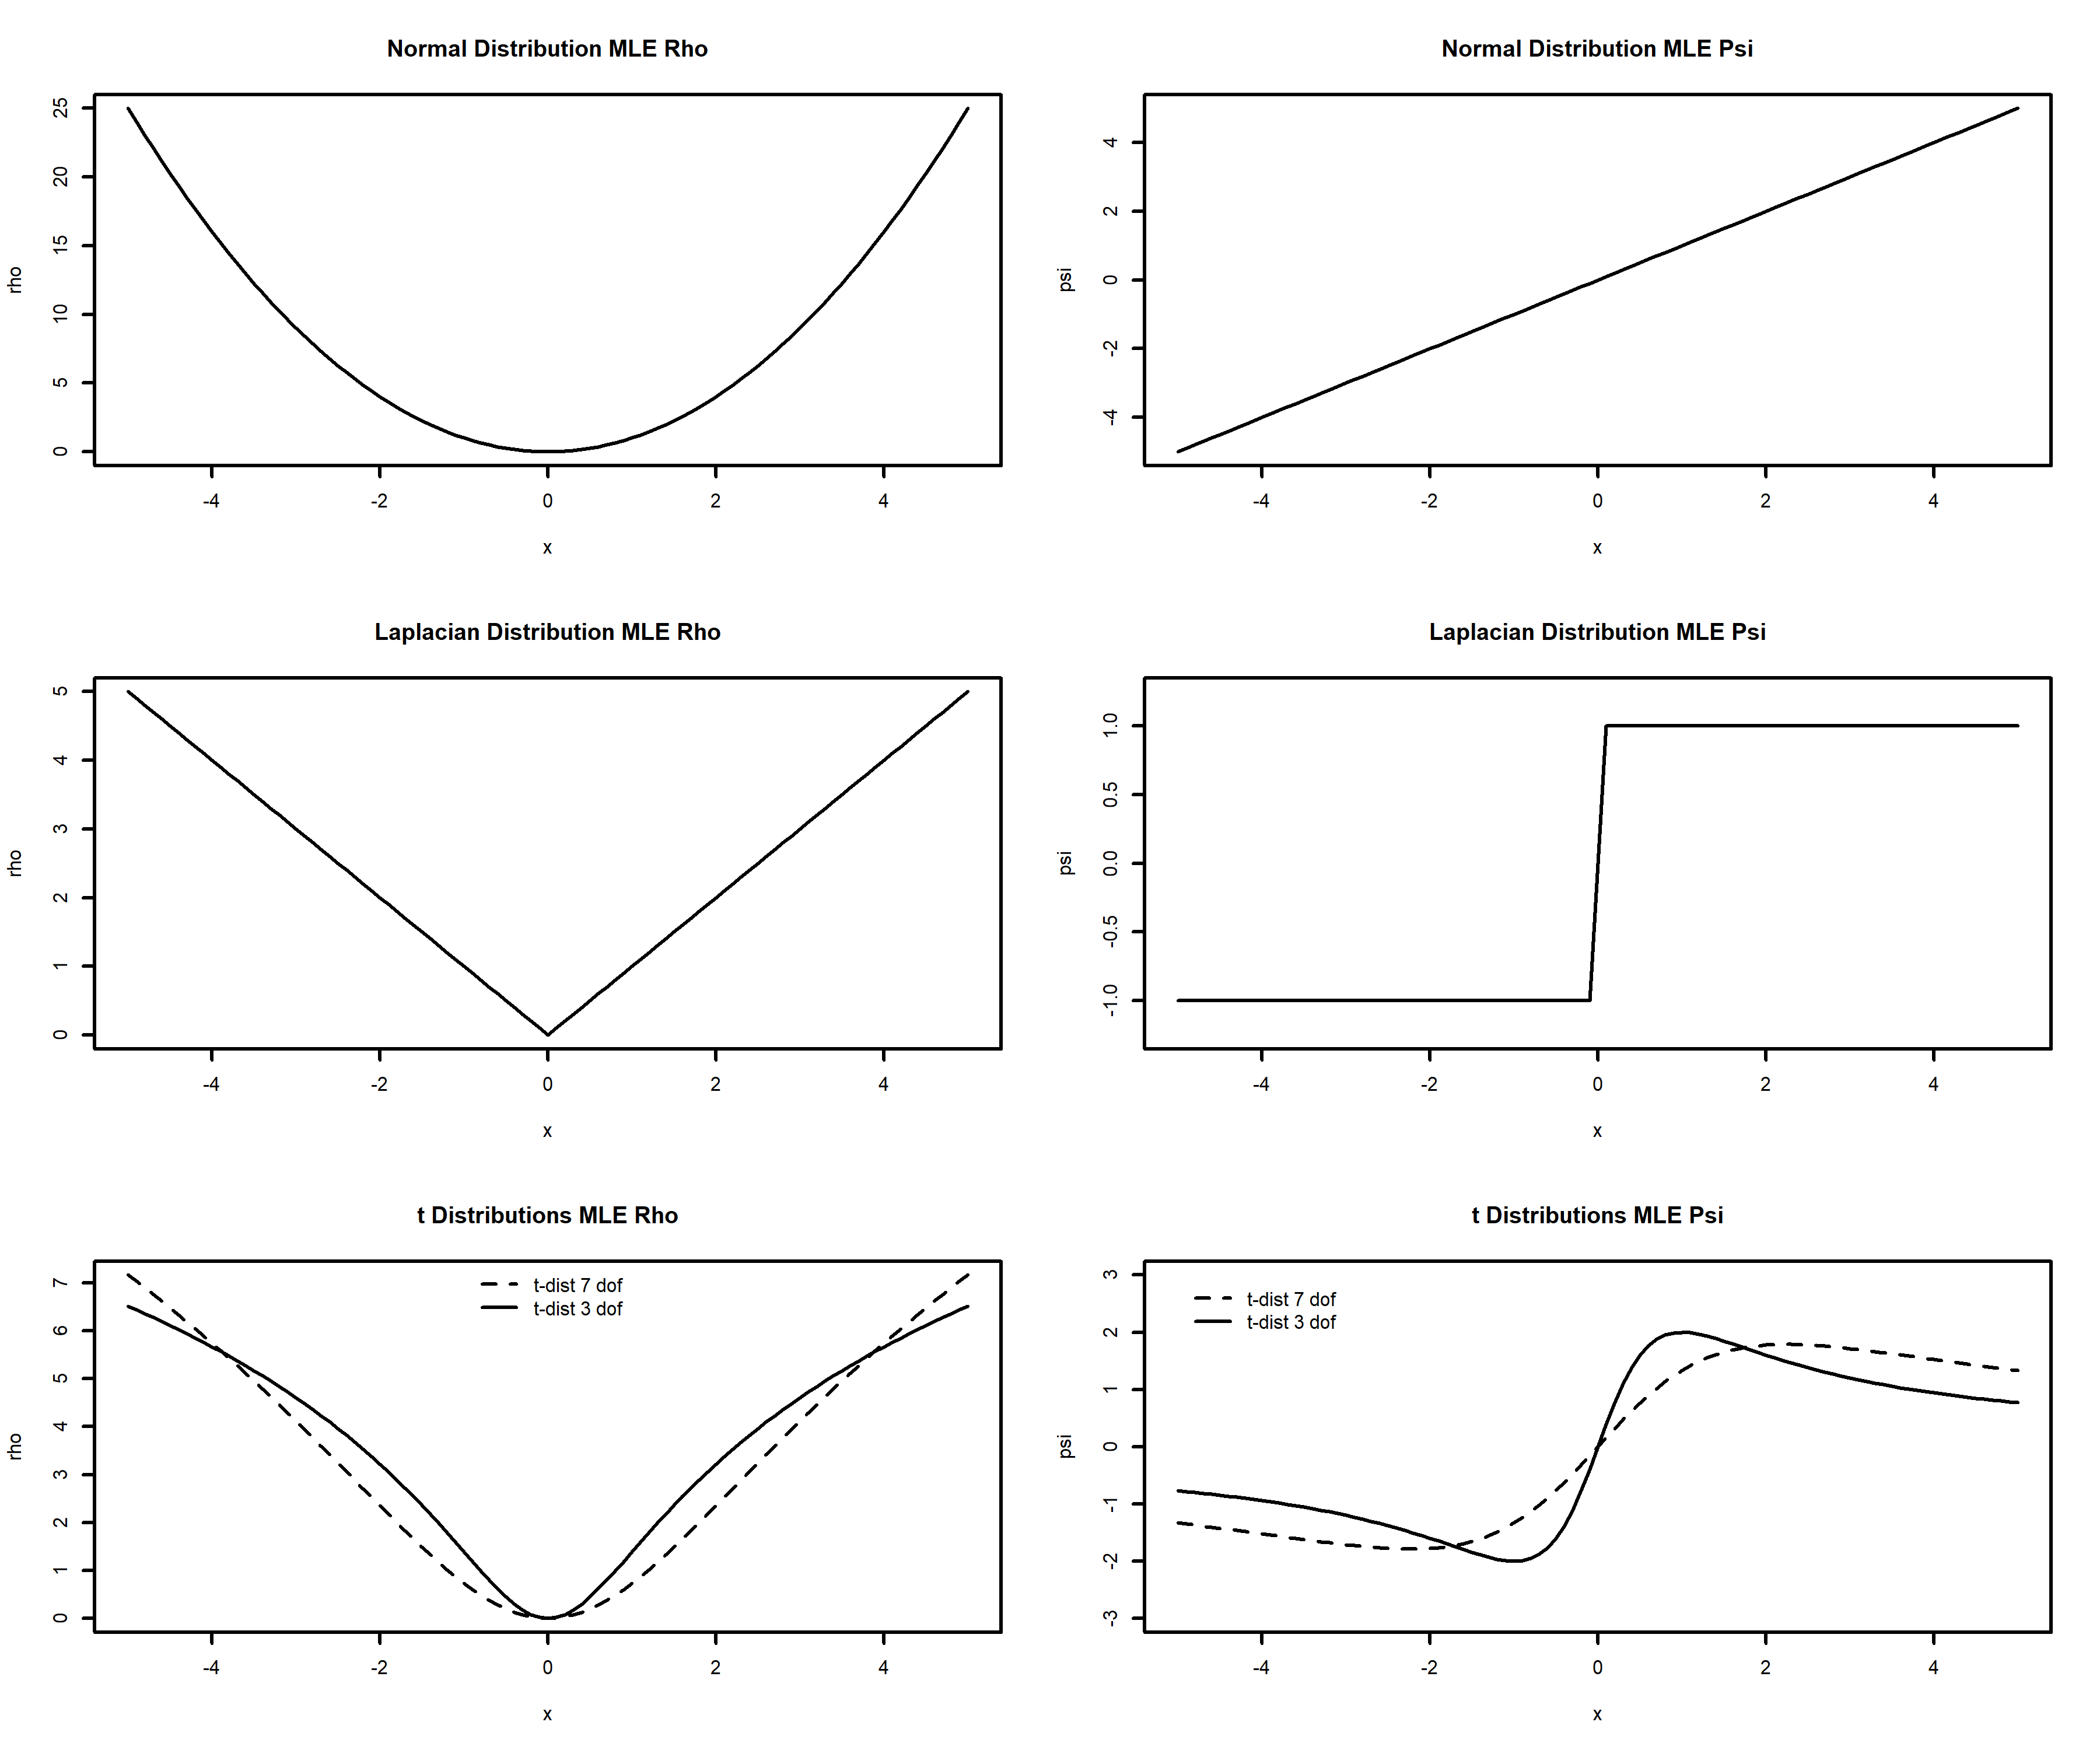
\includegraphics[scale=1.1]{1C__Users_tkpme_Dropbox_BookPCRA_Springer_Produ___B_Prob___Stat_for_PCRM_Plots_mleRhoPsiPlots.png}
\par\end{centering}
\caption{MLE Loss Functions ($\rho$) and Score Functions ($\psi$) for Normal,
Laplacian, and t-Distributions}

\label{fig: mleRhoPsiPlots}
\end{figure}


\subsection{Regression Model MLEs\label{subsec:RegressionModelMLEs}}

We next extend our results on MLEs to cross--section regression models.
We focus on the cross--section model for a single time period with
the time subscript $t$ dropped, but keep in mind that the model will
be fit for each time period $t$ in some time window:
\begin{align}
r_{i} & =f_{o}\,+\,\beta_{i1}\,\cdot\,f_{1}\,+\,\beta_{i2}\,\cdot\,f_{2}\,+\,\cdots\,+\,\beta_{iK}\,\cdot\,f_{K}\,+\,\varepsilon_{i},\ i=1,\,2,\,\cdots\,,\,N.\label{eq: linRegModNoVectors}
\end{align}
Let $\mathbf{B}$ be the $N\times(K+1)$ matrix whose $i^{th}$ row
is $\mathbf{b}_{i}^{\prime}=(1,\,\beta_{i1},\,\beta_{i2},\,\cdots\,,\beta_{iK})$
and let $\mathbf{f}=(f_{o},\,f_{1},\,\cdots\,,\,f_{K})^{\prime},$
Then the above model may be written more compactly as:
\begin{equation}
r_{i}=\mathbf{b}_{i}^{\prime}\mathbf{f}\,+\,\varepsilon_{i},\ i=1,2,\cdots,N.\label{eq: linRegMod}
\end{equation}

In the above model the $\beta_{ik}$ are fixed predictor variables
and the $f_{k}$ are unknown coefficients, and for this single time--period
model the $f_{k}$ can be considered as unknown regression coefficient
parameters, with $f_{o}$ being the intercept\footnote{In practice, the cross--section factor models are fit for each time
period $t$, and the resulting $f_{k\,t}$ are treated as random variables
that define random time series as time $t$ evolves. This aspect is
discussed further in \CrossSectionalFactorModelsChapter.}. We make the standard assumption that the errors $\varepsilon_{i}$
are independent and identically distributed (i.i.d.) random variables
that are also independent of the $\beta_{ik}$, and further assume
that they have a pdf of the scale family form
\begin{equation}
p(\epsilon)=\frac{1}{s}p_{0}\left(\frac{\epsilon}{s}\right),\ s>0\label{eq: pdfScaledEpsilon}
\end{equation}
where $p_{0}$ is a standard symmetric density such as a standard
normal or standard Laplacian distribution. Using \eqref{eq: linRegMod},
we have
\begin{equation}
p(\epsilon_{i})=\frac{1}{s}p_{0}\left(\frac{r_{i}\,-\,\mathbf{b}_{i}^{\prime}\mathbf{f}}{s}\right),\label{eq: regObsPdf}
\end{equation}
and since the $\epsilon_{i}$ are i.i.d., the joint probability density
$f(\mathbf{r};\,\mathbf{f},\,s)$ of the observations $\mathbf{r}=(r_{1},\,r_{2},\,\cdots\,,\,r_{n})$
is 
\begin{align}
f(\mathbf{r};\,\mathbf{f},\,s) & =\prod_{i\,=\,1}^{N}\frac{1}{s}p_{0}\left(\frac{r_{i}\,-\,\mathbf{b}_{i}^{\prime}\mathbf{f}}{s}\right).\label{eq: regJointObsPdf}
\end{align}

It follows that the log--likelihood function, $l(\mathbf{f},s)$,
is:
\begin{align}
l(\mathbf{f},\,s) & =\ln\,L(\mathbf{f},\,s)\nonumber \\
 & =-N\,\cdot\,\ln(s)\,+\,\sum_{i\,=\,1}^{N}\ln p_{0}\left(\frac{r_{i}\,-\,\mathbf{b}_{i}^{\prime}\mathbf{f}}{s}\right),\label{eq: regLogLikelihood}
\end{align}
which is virtually identical to \eqref{eq:JointMLEmuSigma}. 

The maximum likelihood estimates $(\hat{\mathbf{f}},\,\hat{s})_{mle}$
are the values of $(\mathbf{f},\,s)$ that maximize the above log--likelihood,
and we write this as:
\begin{equation}
(\hat{\mathbf{f}},\,\hat{s})_{mle}=\underset{\mathbf{f},\,s}{\mathrm{argmax}}\left(-N\cdot\ln(s)\,+\,\sum_{i\,=\,1}^{N}\ln p_{0}\left(\frac{r_{i}\,-\,\mathbf{b}_{i}^{\prime}\mathbf{f}}{s}\right)\right).\label{eq: regJointMLE}
\end{equation}

Once again, we explore the impact of non--normal $p_{0}(\epsilon)$
on the linear regression MLE by acting as if $s$ is known, and consider
the optimization only with respect to $\mathbf{f}$. By analogy to
\eqref{eq:MLEsknown} and \eqref{eq: MLEasLossFunction} we can write:
\begin{equation}
\hat{\mathbf{f}}_{mle}=\underset{\mathbf{f}}{\mathrm{argmin}}\left(-\sum_{i=1}^{N}\ln p_{0}\left(\frac{r_{i}\,-\,\mathbf{b}_{i}^{\prime}\mathbf{f}}{s}\right)\right),\label{eq: regMLEsknown}
\end{equation}
and 
\begin{equation}
\hat{\mathbf{f}}_{mle}=\underset{\mathbf{f}}{\mathrm{argmin}}\left(\sum_{i=1}^{N}\rho\left(\frac{r_{i}\,-\,\mathbf{b}_{i}^{\prime}\mathbf{f}}{s}\right)\right),\label{eq: regMLEasLossMin}
\end{equation}
where $\rho(x)=-\ln\,p_{0}(x)$.

By taking the derivative of the right hand side of \eqref{eq: regMLEasLossMin}
with respect to $\mathbf{f}$, and setting it equal to zero, we can
characterize $\hat{\mathbf{f}}_{mle}$ as the solution of the estimating
equation
\begin{equation}
\sum_{i=1}^{N}\mathbf{b}_{i}\psi\left(\frac{r_{i}\,-\,\mathbf{b}_{i}^{\prime}\mathbf{f}}{s}\right)=0\label{eq: regMLEestEqn}
\end{equation}
where $\psi(x)=\frac{d}{dx}\rho(x)$.

We now discuss three possible error distribution choices in terms
of the pdf $p_{0}(\epsilon)$, and their corresponding regression
estimators.
\begin{example}
Normal Distribution Regression MLE

In the case, the density $p_{0}$ is the standard normal pdf, and
as \eqref{eq: regMLEasLossMin} does not depend upon $s$, the result
is the least--squares (LS) estimate
\begin{align}
\hat{\mathbf{f}}_{mle,\,normal} & =\hat{\mathbf{f}}_{LS}=\underset{\mathbf{f}}{\mathrm{argmin}}\left(\sum_{i\,=\,1}^{N}(r_{i}\,-\,\mathbf{b}_{i}^{\prime}\,\mathbf{f})^{2}\right),\label{eq: LSminimization}
\end{align}
and \eqref{eq: regMLEestEqn} becomes the corresponding LS normal
equations:
\begin{equation}
\sum_{i\,=\,1}^{N}\mathbf{b}_{i}\left(r_{i}\,-\,\mathbf{b}_{i}^{\prime}\,\hat{\mathbf{f}}_{LS}\right)=\mathbf{0}.\label{eq: LSnormalEqns}
\end{equation}

Laplacian Distribution Regression MLE

In this case, $p_{0}$ is the Laplacian pdf, so that the resulting
regression estimator is the Least--Absolute--Deviation (LAD) estimator:
\begin{align}
\hat{\mathbf{f}}_{mle,\,Laplacian} & =\hat{\mathbf{f}}_{LAD}=\underset{\mathbf{f}}{\mathrm{argmin}}\left(\sum_{i\,=\,1}^{N}|r_{i}\,-\,\mathbf{b}_{i}^{\prime}\mathbf{f}|\right).\label{eq: LADminimization}
\end{align}
The \emph{LAD} estimator is also known as the \emph{L1} estimator,
and good numerical methods for solving the \emph{LAD/L1} minimization
problem \eqref{eq: LADminimization} are widely available in both
commercial and open source software packages.

t--Distribution Regression MLE

In this case we assume that $p_{0}$ is the standard t--distribution
pdf with known parameter $\nu$, and the t--distribution regression
MLE minimization problem becomes
\begin{equation}
\hat{\mathbf{f}}_{mle,\,tdist}=\underset{\mathbf{f}}{\mathrm{argmin}}\left(\sum_{i\,=\,1}^{N}\log\left(1\,+\,\dfrac{1}{\nu}\left(\frac{r_{i}\,-\,\mathbf{b}_{i}^{\prime}\mathbf{f}}{s}\right)^{2}\right)\right).
\end{equation}
As in the case of Example \eqref{exa:tDistributionMLE}, the above
is a non--convex optimization problem that is not easily solved in
closed form, though some of the powerful numerical solution techniques
described in \RobustMethodsChapter\ and \citet{AzzaliniCapitanio2014}
have applicability to this problem as well.
\end{example}

\subsubsection*{Error Distribution Tail Fatness and Shapes of MLE Rho and Psi Functions}

It is important to note the relationship between the fatness of the
tail of the error distributions, and the shapes of the $\rho(x)$
and $\psi(x)$ functions. For the normal distributions, $\rho_{mle,\,normal}(x)$
is quadratic and grows very rapidly, while $\psi_{mle,\,normal}(x)=x$
is increasing and unbounded. For Laplacian distributions, which are
more fat--tailed than normal distributions, $\rho_{mle,\,exp}(x)=|x|$
grows only linearly but is unbounded, and $\psi_{mle,\,exp}(x)=sgn(x)$
is non--decreasing and bounded. For t--distributions, which are
more fat--tailed than the Laplacian distribution, $\rho_{mle,\,tdist}(x)$
grows only logarithmically (slower than linear) but is still unbounded,
and $\psi_{mle,\,tdist}(x)$ is not only bounded but is also non--monotonic
and decreases to zero as $x$ tends to plus and minus infinity.

\subsubsection*{Joint MLE of Regression and Scale Parameters}

Computing the joint MLEs $\hat{\mathbf{f}}_{mle}$ and $\hat{s}_{mle}$
of the regression and scale parameters is in general a complex nonlinear
optimization for non--normal error distributions such as the t--distribution.
However, in the case of the normal and Laplacian distributions, it
is straightforward to derive formulas for the joint MLEs. For the
normal distribution, $\hat{s}_{mle,\,normal}$ is the square root
of the sample average of the squared residuals $\hat{\epsilon}_{i}=r_{i}-\mathbf{b}_{i}^{\prime}\hat{\mathbf{f}}_{mle,\,normal}$
. For Laplacian distributions, $\hat{s}_{mle,\,exp}$ is the sample
average of the absolute value of the residuals $\hat{\epsilon}_{i}=r_{i}-\mathbf{b}_{i}^{\prime}\hat{\mathbf{f}}_{mle,\,normal}$
.

\subsubsection*{The Maximum Likelihood Principle and Asymptotic Optimality of MLEs}

This \emph{maximum--likelihood principle} asserts that if one knows
the data distribution then one should use a maximum--likelihood estimator.
Although this is only a reasonableness principle that is commonly
invoked in the case of finite--sample estimators, it has the benefit
of the following asymptotic optimality property: if the data is generated
by an assumed distribution, then the MLE based on that distribution
has an asymptotic variance that is the smallest asymptotic variance
achievable by a consistent estimator. For a given distribution there
is an analytic expression for that minimum variance, called the information--inequality
lower bound. The formula for the lower bound is given in TS \ref{sec: Fisher Info =000026 MLE Optimality}. 

Maximum Likelihood Estimators generalize naturally to outlier--resistant
robust estimators, and the similarities between the problem formulations
in Section \ref{sec: MLEs} and \RobustMethodsChapter\ are striking.
In fact, a regression M-estimator is best viewed as an outlier-resistant
generalization of the regression MLE equations \eqref{eq: regMLEasLossMin}
and \eqref{eq: regMLEestEqn}.

\subsection{Covariance Matrix MLEs}

The sample covariance matrix estimator is known to be a maximum likelihood
estimator when the return vectors ${\bf r}_{t}=\left(r_{t1},\,...\,,\,r_{tN}\right)^{\prime},\ t=1,\,,2,\,\cdots,\,T$
are multivariate normal. The proof, however, is fairly complex and
is typically covered only in multivariate statistics courses. Maximum--likelihood
estimators for the case of non--normal multivariate elliptical distributions
are discussed in \CrossSectionalFactorModelsChapter.

\section{Useful Inequalities}

\uline{Markov's Inequality}

If $X$ is any non--negative random variable ($X\geqslant0$), and
$a$ is a positive constant, then:
\begin{equation}
P(X\geqslant a)\leqslant\dfrac{\mathrm{E}\left[X\right]}{a},\,a>0.\label{eq: MarkovInequality}
\end{equation}

\uline{Moment Bound}

Markov's Inequality is easily extended to higher moments of $X$.
If $X$ is any non--negative random variable, and if $a$ and $r$
are positive constants, then:.

\begin{equation}
P(X\geqslant a)\leqslant\dfrac{\mathrm{E}\left[X^{r}\right]}{a^{r}},\ a,\,r>0.\label{eq: MomentBound1}
\end{equation}
In particular,
\begin{equation}
P(X\geqslant a)\leqslant\underset{r>0}{\inf}\dfrac{\mathrm{E}\left[X^{r}\right]}{a^{r}},\ a>0.\label{eq: MomentBound2}
\end{equation}

Equation \ref{eq: MomentBound2} is known as the \emph{Moment Bound},
and \citet{PhilipsNelson1995} show that the moment bound is tighter
than Chernoff's Bound for positive tail probabilities.

\uline{Chebyshev's Inequality}

If a random variable $X$ has mean $\mu=\mathrm{E}\left[X\right]$
and variance $\sigma^{2}=\mathrm{E}\left[(X-\mu)^{2}\right]$, and
$b$ is any positive constant, then:
\begin{equation}
P\left(\left|X-\mu\right|\geqslant b\right)\leqslant\dfrac{\sigma^{2}}{b^{2}},\ b>0.\label{eq: ChebyshevInequalityAppB}
\end{equation}

\uline{Chernoff's Bound}

Chernoff's Bound is the tightest general purpose inequality that applies
to random variables whose domain is the entire real line.

\begin{subequations}
\begin{align}
P(X\geqslant a) & \leqslant\underset{\theta>0}{\inf}\dfrac{\mathrm{E}(\exp\left(\theta X\right))}{\exp\left(\theta a\right)}\label{eq: ChernoffsBound1}\\
P(X\leqslant a) & \leqslant\underset{\theta<0}{\inf}\dfrac{\mathrm{E}(\exp\left(\theta X\right))}{\exp\left(\theta a\right)}.\label{eq:ChernoffsBound2}
\end{align}
\end{subequations}

\uline{Jensen's Inequality}

The probabilistic version of Jensen's inequality for the case of a
convex function $g$ is a generalization of the statement that the
secant line of a function lies below the function. Specifically, if
$X$ is a random variable with expected value $\mathrm{E}\left[X\right]$,
and $g$ is a convex function, then
\begin{equation}
g\left(\mathrm{E}\left[X\right]\right)\leqslant\mathrm{E}\left[g(X)\right].\label{eq: JensenInequalityConvexFnc}
\end{equation}
If $g$ is a strictly convex function, then Jensen's inequality is
strict:
\begin{equation}
g\left(\mathrm{E}\left[X\right]\right)<\mathrm{E}\left[g(X)\right].\label{eq: JensenInequalityStrictlyConvexFnc}
\end{equation}
For a concave and strictly concave functions $g$, the above inequalities
are reversed.

\section{Limit Theorems for Random Variables and Distributions}

This section discusses key limit theorems of sequences of random variables
and distribution functions that play a central role in the large sample
asymptotic theory of parameter estimators. For further background
on such asymptotics, the document ``Notes for a graduate level course
in asymptotics for statisticians'' by Professor David R. Hunter (available
at \url{https://sites.math.rutgers.edu/~sg1108/asymp1.pdf}) is highly
recommended.

\subsection{Random Variables Convergence\label{subsec:Random-Variables-Convergence}}

\uline{Convergence in Probability}

An infinite sequence of random variables $X_{1},\,X_{2,}\cdots$ \emph{converges
in probability} to a random variable $X$ if for every $\epsilon>0$
the following limit condition holds
\begin{equation}
\underset{n\rightarrow\infty}{\lim}P\left(|X_{n}\,-\,X|<\epsilon\right)=1,\label{eq: convInProbDef}
\end{equation}
and in that case we write
\begin{equation}
X_{n}\overset{p}{\rightarrow}X.
\end{equation}
Sometimes $X$ will be a constant $X=c$, and frequently the random
variables $X_{n}$ are parameter estimates $X_{n}=\hat{\theta}_{n}$.

\uline{Weak Law of Large Numbers}

If $X_{1},\,X_{2,}\cdots$ are independent and identically distributed
with finite mean $\mu=\mathrm{E}(X_{1})$, then the sample mean $\overline{X}_{n}=\dfrac{1}{n}\sum_{i\,=\,1}^{n}X_{i}$
converges in probability to $\mu$:
\begin{equation}
\overline{X}_{n}\overset{p}{\rightarrow}\mu.\label{eq: WLLN}
\end{equation}
The proof of the result as stated is involved. But a proof under the
assumption that the $X_{i}$ have finite variance $\sigma^{2}$, which
is often a reasonable assumption, is an easy consequence of Chebychev's
inequality.\textbf{ }Additionally, it is not hard to show that for
i.i.d. $X_{i}$ with finite variance $\sigma^{2}$, the quantity $n^{-1}\sum_{i\,=\,1}^{n}(X_{i}\,-\,\mu)^{2}$
converges in probability to $\sigma^{2}$.

\subsection{Convergence in Distribution}

Let the infinite sequence of random variables $X_{1},\,X_{2},\,\cdots$
have cumulative distribution functions $F_{1}(x),\,F_{2}(x),\cdots,$and
let $X$ have cumulative distribution function $F(x)$, and let $C$
be the set of points of continuity of $F(x)$. The sequence $X_{1},\,X_{2,}\,\cdots$
is said to \emph{converge in distribution} $X$ if
\begin{equation}
\underset{n\,\rightarrow\,\infty}{lim}F_{n}(x)=F(x),\,x\in C\label{eq: convInDist}
\end{equation}
and one writes this as:
\begin{equation}
X_{n}\overset{d}{\rightarrow}X\quad\mathrm{or}\quad X_{n}\overset{d}{\rightarrow}F.
\end{equation}
NOTE: For our purposes in this book the reader will only need the
above two types of convergence of random variables. However, there
are other modes of convergence of random variables, e.g., convergence
almost surely and convergence in mean, and the interested reader can
find a good discussion of these in the Hunter reference given at the
beginning of this section.

\subsection{Slutsky's Theorem}

If $X_{1},\,X_{2}\cdots$ and $Y_{1},\,Y_{2}\cdots$ are infinite
sequences of random variables such that $X_{n}\overset{d}{\rightarrow}X$
and $Y_{n}\overset{p}{\rightarrow}c$, where $c$ is a constant, then:
\[
X_{n}\,+\,Y_{n}\,\overset{d}{\rightarrow}\,X\,+\,c,\qquad X_{n}Y_{n}\,\overset{d}{\rightarrow}\,cX\qquad X_{n}/Y_{n}\,\overset{d}{\rightarrow}\,X/c,\:\mathrm{provided}\,c\ne0.
\]


\subsection{Central Limit Theorem (CLT)}

Let $X_{1},\,X_{2,}\,\cdots$ be an infinite sequence of independent
and identically distributed (i.i.d.) random variables with finite
mean $\mu$, finite variance $\sigma^{2}$, and let $\overline{X}_{n}$
be the sample mean of the $X_{i}$ for a sample of size $n$. There
exist a number of sophisticated \emph{central limit theorems} (CLTs)
asserting the asymptotic normality of the sample mean, the simplest
of which is the following classical CLT:
\begin{equation}
\sqrt{n}\left(\overline{X}_{n}\,-\,\mu\right)\,\overset{d}{\rightarrow}\,N\left(0,\,\sigma^{2}\right)\quad\mathrm{or}\quad\sqrt{n}\left(\overline{X}_{n}\,-\,\mu\right)\,\overset{d}{\rightarrow}\,Y\label{eq: CLTv1}
\end{equation}
where $Y$ is normally distributed with mean zero and variance $\sigma^{2}$.
Equivalently, this CLT can be stated as:
\begin{equation}
\sqrt{n}\,\dfrac{\overline{X}\,-\,\mu}{\sigma}\,\overset{d}{\rightarrow}\,N\left(0,\,1\right).\label{eq: CLTv2}
\end{equation}


\section{Estimator Asymptotic Results and Their Use}

\subsection{Consistent Estimators\label{subsec: estConsistent}}

A \emph{consistent} estimator $\hat{\theta}_{n}$ is one that \emph{converges
in probability} to the true but unknown parameter value $\theta$
as the sample size $n$ goes to infinity, and we write this property
of an estimator as:
\begin{equation}
\hat{\theta}_{n}\,\stackrel{p}{\rightarrow}\,\theta.\label{eq: convInProb}
\end{equation}
We provide a precise mathematical definition of convergence in probability
in Section \ref{subsec:Random-Variables-Convergence}, but a verbal
description of this property is as follows: as the sample size tends
to infinity, the probability that $\left|\hat{\theta}_{n}\,-\,\theta\right|$
is smaller than any specified positive amount converges to 1.

Most estimators commonly used in practice are consistent under standard
assumptions. For example, the sample mean is a consistent estimator
of the mean $\mu$, the sample variance estimators $\hat{\sigma}_{n}^{2}$
and $S_{n}^{2}$ are both consistent estimators of the variance $\sigma^{2}$,
and the sample standard deviation estimator $\hat{\sigma}_{n}$ is
a consistent estimator of the standard deviation $\sigma$.

\subsection{Estimator Asymptotic Variance\label{subsec: estAsympVariance}}

Consider the sample mean
\[
\overline{r}_{n}=\frac{1}{n}\sum_{t\,=\,1}^{n}r_{t}
\]
based on on uncorrelated returns $r_{t},\:t=1,\,2,\,\ldots\,,\,n$
with a common mean $\mu$ and common variance $\sigma^{2}$. When
the context is clear we will drop the subscript $n$ on $\overline{r}_{n}$.
It is well known that the finite sample variance of $\overline{r}_{n}$
is
\[
V_{n}\left(\overline{r}\right)=\mathrm{var}(\overline{r})=\frac{\sigma^{2}}{n}.
\]
and so the variance of the sample mean goes to zero at rate $1/n$.

Most well--known estimators have a variance that converges to zero
at a rate $1/n$ under standard assumptions. For example, the sample
median, sample covariance, sample correlation coefficient, and regression
coefficient estimators, among many others, have variances that decrease
at a rate $1/n$. For any such estimator $\hat{\theta}_{n}$, one
can obtain an ``asymptotic variance'' by applying a multiplicative
factor $\sqrt{n}$ to the estimator in an appropriate manner. For
example, in the case of the sample mean $\overline{r}_{n}$ one has
$\mathrm{var}\left(\sqrt{n}\,\overline{r}_{n}\right)=\sigma^{2}$
for every sample size $n$.

If an estimator $\hat{\theta}_{n}$ is a consistent estimator of a
parameter $\theta$, then under certain standard conditions satisfied
by most estimators encountered in practice, the distribution of the
standardized estimator $\sqrt{n}\left(\hat{\theta}_{n}\,-\,\theta\right)$
converges in distribution to a normal distribution that has mean zero
and an asymptotic variance $V\left(\theta;\,\hat{\theta}_{n}\right)$,
which is written as
\begin{equation}
\sqrt{n}\left(\hat{\theta}_{n}\,-\,\theta\right)\,\overset{d}{\rightarrow}\,N\left(0,\,V\left(\theta;\,\hat{\theta}_{n}\right)\right).\label{eq: sqrtnStandardizedEstimator}
\end{equation}

The argument $\hat{\theta}_{n}$ in $V\left(\theta;\,\hat{\theta}_{n}\right)$
reflects that fact that the asymptotic variance depends on the choice
of estimator, and when the context makes it clear which estimator
is being considered, the asymptotic variance is written more simply
as $V\left(\theta\right)$.
\begin{example}
Asymptotic Variance of the Sample Variance Estimator
\end{example}
If i.i.d. returns $r_{i}$ have a finite fourth moment, then it turns
out that the asymptotic variance of the sample variance estimator
$\hat{\sigma}_{n}^{2}=\frac{1}{n}\sum_{i\,=\,1}^{n}\left(r_{i}\,-\,\bar{r}_{n}\right)^{2}$
is given by
\begin{equation}
V(\hat{\sigma}_{n}^{2})=\mathrm{var}\left[\left(r_{1}\,-\,\mu\right)^{2}\right]=\mu_{4}\,-\,\sigma^{4}\label{eq: asympVarianceSampleVariance}
\end{equation}
where $\mu_{4}=\mathrm{E}\left[(r\,-\,\mu)^{4}\right]$ is the fourth
central moment. A proof of the this result is as follows.

Let $a=\mathrm{var}\left(r_{1}\,-\,\mu\right)^{2}$, and note that:
\begin{align*}
a & =\mathrm{E}\left[(r_{1}\,-\,\mu)^{4}\right]\,-\,\mathrm{E}^{2}\left[(r_{1}\,-\,\mu)^{2}\right]\\
 & =\mu_{4}\,-\,\sigma^{4}.
\end{align*}

Since subtracting $\mu$ from both $r_{i}$ and $\bar{r}$ does not
change the distribution of $r_{i}-\bar{r}$, we can assume the mean
of the $r_{i}$ is zero. Consequently
\begin{align*}
\frac{1}{n}\sum_{i\,=\,1}^{n}\left(r_{i}\,-\,\bar{r}_{n}\right)^{2} & =\frac{1}{n}\,\sum_{i\,=\,1}^{n}r_{i}^{2}\,-\,\frac{2}{n}\,\sum_{i\,=\,1}^{n}r_{i}\bar{r}_{n}\,+\,\bar{r}_{n}^{2}\\
 & =\frac{1}{n}\,\sum_{i\,=\,1}^{n}r_{i}^{2}\,-\,\bar{r}_{n}^{2}.
\end{align*}
and recalling that the mean of the $r_{i}$ is zero, we have.
\[
\sqrt{n}\left(\hat{\sigma}_{n}^{2}\,-\,\sigma^{2}\right)=\sqrt{n}\left(\frac{1}{n}\,\sum_{i\,=\,1}^{n}r_{i}^{2}\,-\,\sigma^{2}\right)\,-\,\sqrt{n}\,\bar{r}_{n}^{2}.
\]

It follows from the CLT that the first term on the right converges
in distribution to a $N(0,\,a)$ distribution. Furthermore, the second
term can be written as $\bar{r}_{n}\,\sqrt{n}\,\bar{r}_{n}$, and,
by the CLT, $\sqrt{n}\,\bar{r}_{n}\stackrel{d}{\rightarrow}Z$ where
$Z$ is a $N(0,1)$ random variable, and $\bar{r}_{n}$ converges
in probability to $c=0$. By Slutsky's Theorem the right hand side
of the above equation converges to a $N(0,\,a)$ distribution.

\textbf{}

\section{Delta Methods}

We first discuss the univariate delta method that allows one to obtain
the asymptotic variance of a nonlinear transformation of an estimator,
a leading example of which is obtaining the asymptotic variance of
a sample volatility estimator from the asymptotic variance of a sample
variance estimator. We then discuss the bivariate delta method that
that allows one to obtain the asymptotic variance of a performance
estimator that is the ratio of two estimators based on the same set
of returns, e.g., the Sharpe ratio and Sortino ratio, from the asymptotic
$2\times2$ covariance matrix of the individual estimators for the
numerator and denominator.

\subsection{Univariate Delta Method}

Suppose we have a formula $V(\theta)=V(\theta;\,\hat{\theta}_{n})$
for the asymptotic variance of a consistent estimator $\hat{\theta}_{n}$,
and want to find the variance $V\left(\theta;\,g\left(\hat{\theta}_{n}\right)\right)$
of a nonlinear transformation $g\left(\hat{\theta}_{n}\right)$ of
$\hat{\theta}_{n}$, where the function $g(t)$ has a continuous first
derivative $g^{\prime}(t)$. Using the Mean Value Theorem  gives
\begin{equation}
g\left(\hat{\theta}_{n}\right)=g(\theta)\,+\,g^{\prime}(\theta^{*})\,\cdot\,\left(\hat{\theta}_{n}\,-\,\theta\right),\ \mathrm{where}\:\theta^{*}\:\mathrm{lies}\ \mathrm{between}\ \theta\ \mathrm{and}\ \hat{\theta}_{n}.\,\label{eq:UnivariateDeltaStep1}
\end{equation}
It follows that
\begin{equation}
\sqrt{n}\left(g\left(\hat{\theta}_{n}\right)\,-\,g(\theta)\right)=g^{\prime}(\theta^{*})\,\cdot\,\sqrt{n}\left(\hat{\theta}_{n}\,-\,\theta\right),\ \mathrm{with}\:\theta^{*}\ \mathrm{between}\ \theta\ \mathrm{and}\ \hat{\theta}_{n}.\label{eq:UnivariateDeltaStep2}
\end{equation}
Taking the limit on the right hand side as $n\,\rightarrow\,\infty$,
the consistency of $\hat{\theta}_{n}$ for $\theta$ implies that
$\theta^{*}\,\stackrel{p}{\rightarrow}\,\theta$ and $g(\theta^{*})\,\stackrel{p}{\rightarrow}\,g(\theta)$
as $n\,\rightarrow\,\infty$, and so the right hand side converges
to $g^{\prime}(\theta)\,\cdot\,Y$, where $Y$ has mean zero and variance
$V(\theta)$. Thus by Slutsky's Theorem, the right hand side converges
to a random variable with mean zero and variance $\left[g^{\prime}(\theta)\right]^{2}\,\cdot\,V(\theta)$.
It follows that the asymptotic variance of the left hand side above
is:
\begin{equation}
V\left(\theta;\,g\left(\hat{\theta}_{n}\right)\right)=\left[g^{\prime}(\theta)\right]^{2}V(\theta).
\end{equation}

\begin{example}
Volatility Estimator Asymptotic Variance

Since volatility is related to variance through the square root transformation
$\sigma=\sqrt{\sigma^{2}}$, the transformation $g(t)=t^{1/2}$ and
$g^{\prime}(t)=t^{-1/2}/2$. With $t=\theta=\sigma^{2}$ we have $\left[g^{\prime}(\theta)\right]^{2}=\nicefrac{1}{\,4\,\sigma^{2}}$
and use of the formula \eqref{eq: asympVarianceSampleVariance} for
the asymptotic variance of the sample variance gives:
\begin{equation}
V(\sigma;\,\hat{\sigma}_{n})=\dfrac{\mu_{4}\,-\,\sigma^{4}}{4\sigma^{2}}.\label{eq: asympVarianceVolEst}
\end{equation}
\end{example}

\subsection{The Bivariate Delta Method}

Performance estimators such as the Sharpe ratio, the Sortino ratio,
and the Information ratio, are ratios of two estimators, and for the
purpose of the discussion here, it is assumed that both estimators
use the same set of i.i.d. returns $r_{1},\,r_{2},\,\cdots\,,\,r_{n}$.
For example, the Sharpe ratio estimator is
\begin{equation}
\widehat{\mathrm{SR}}=\dfrac{\hat{\mu}_{e}}{\hat{\sigma}}=\dfrac{\hat{\mu}\,-\,r_{f}}{\hat{\sigma}}\label{eq: SRestimator}
\end{equation}
where $\hat{\mu}$ is the sample mean, and $\hat{\sigma}$ is the
sample variance, of the set of returns. For purposes of the discussion
here, it is assumed that the $r_{i}$ are independent and identically
distributed.

A performance ratio estimator $\widehat{\mathrm{PR}}$ in general
has the form
\[
\widehat{\mathrm{PR}}=\dfrac{\hat{\theta}_{1}}{\hat{\theta}_{2}}
\]
where $\hat{\theta}_{1}$ and $\hat{\theta}_{2}$ are two estimators
based on the same set of returns. The asymptotic variance of such
an estimator can be computed using the following bivariate delta method,
which is an extension of the univariate delta method in the previous
sub--section.

Let $\butheta=(\theta_{1},\,\theta_{2})^{\prime}$ and let $g(\butheta)=g(\theta_{1},\,\theta_{2})$
be a scalar--valued transformation of $\butheta$. Then given a bivariate
estimator $\hat{\butheta}=(\hat{\theta}_{1},\,\hat{\theta}_{2})^{\prime}$,
one obtains the estimator $\widehat{g(\butheta)}=g(\hat{\theta}_{1},\,\hat{\theta}_{2})$
of $g(\butheta)$. For example, in the case of the Sharpe ratio:
\begin{equation}
g(\butheta)=\dfrac{\theta_{1}}{\sqrt{\theta_{2}}}\quad\mathrm{with}\quad\theta_{1}=\mu_{e},\:\theta_{2}=\sigma^{2}.\label{eq: gThetaSharpeRatio}
\end{equation}

A Taylor series expansion of $\widehat{g(\butheta)}$ about the true
value $\butheta$ gives:
\[
\widehat{g(\butheta)}=g(\butheta)\,+\,\dfrac{\partial g(\butheta)}{\partial\theta_{1}}\left(\hat{\theta}_{1}\,-\,\theta_{1}\right)\,+\,\dfrac{\partial g(\butheta)}{\partial\theta_{2}}\left(\hat{\theta}_{2}\,-\,\theta_{2}\right)\,+\,Rem_{n}
\]
where the estimates are based on i.i.d. returns $r_{1},\,r_{2},\,\cdots\,,\,r_{n}$,
and the remainder $Rem_{n}$ can be shown to go to zero faster than
$1/\sqrt{n}$ under standard conditions. The asymptotic variance $V_{\hat{g}}=V_{\hat{g}}(\butheta)$
of $\widehat{g(\butheta)}$ is the limiting asymptotic variance of
\[
\sqrt{n}\,\cdot\,\left(\widehat{g(\butheta)}\,-\,g(\butheta)\right)=\dfrac{\partial g(\butheta)}{\partial\theta_{1}}\sqrt{n}\left(\hat{\theta}_{1}\,-\,\theta_{1}\right)\,+\,\dfrac{\partial g(\butheta)}{\partial\theta_{2}}\sqrt{n}\left(\hat{\theta}_{2}\,-\,\theta_{2}\right)\,+\,\sqrt{n}\,\cdot\,Rem_{n}.
\]

Assuming the usual asymptotic joint normality of the estimates $\hat{\theta}_{1}$
and $\hat{\theta}_{2}$, and noting that the remainder term goes to
zero asymptotically, the asymptotic variance of $\widehat{g(\butheta)}$
is:
\begin{equation}
V_{\hat{g}}=\nabla g(\butheta)^{\prime}\,\mathbf{V}_{\butheta}\,\nabla g(\butheta)\label{eq: ghatVariance}
\end{equation}
where $\mathbf{V}_{\butheta}$ is the asymptotic covariance matrix
of the estimator $\hat{\butheta}=(\hat{\theta}_{1},\,\hat{\theta}_{2})^{\prime}$:
\begin{equation}
\mathbf{V}_{\butheta}=\left(\begin{array}{ll}
\mathrm{var}_{\infty}(\hat{\theta}_{1}) & \ \mathrm{cov}_{\infty}(\hat{\theta}_{1},\,\hat{\theta}_{2})\\
\mathrm{cov}_{\infty}(\hat{\theta}_{1},\,\hat{\theta}_{2}) & \ \mathrm{var}_{\infty}(\hat{\theta}_{2})
\end{array}\right).\label{eq: VthetaCovMat}
\end{equation}

For estimators $\hat{\theta}_{1}$ and $\hat{\theta}_{2}$ that are
sums of non--linear functions of i.i.d. returns, the above asymptotic
variances and covariances can be computed from a single term of each
of the two summations. This is the case in the following example.
\begin{example}
The Sharpe Ratio Asymptotic Variance Using the Bivariate Delta Method.
\end{example}
For the Sharpe ratio we have $\hat{\theta}_{1}=\bar{r}\,-\,r_{f}=\dfrac{1}{n}\,\sum_{t\,=\,1}^{n}r_{i}\,-\,r_{f}$
and $\hat{\theta}_{2}=\dfrac{1}{n}\,\sum_{t\,=\,1}^{n}(r_{i}\,-\,\bar{r})^{2}$.
The asymptotic variance of $\hat{\theta}_{1}$ is $\sigma^{2}$, and
from \eqref{eq: asympVarianceSampleVariance} we know that the asymptotic
variance of $\hat{\theta}_{2}$ is $\mu_{4}\,-\,\sigma^{4}$. The
asymptotic covariance between $\hat{\theta}_{1}$ and $\hat{\theta}_{2}$
is easily shown to be $\mu_{3}=\mathrm{E}\left[(r_{1}\,-\,\mu)^{3}\right]$.
Thus
\[
\mathbf{V}_{\butheta}=\left(\begin{array}{ll}
\sigma^{2} & \ \mu_{3}\\
\mu_{3} & \ \mu_{4}\,-\,\sigma^{4}
\end{array}\right)
\]

and since for the Sharpe ratio $g(\butheta)$ is given by \eqref{eq: gThetaSharpeRatio},
its gradient is:
\[
\nabla g(\butheta)=\left(\dfrac{1}{\sigma},\,-\dfrac{\mu_{e}}{2\,\sigma^{3}}\right)^{\prime}.
\]

Plugging the above two expressions into \eqref{eq: ghatVariance}
shows that the asymptotic variance of the Sharpe ratio is:
\begin{align}
V_{\widehat{SR}} & =1\,-\,K_{3}\,\cdot\,SR\,+\,\dfrac{K_{4}\,+\,2}{4}\,{SR}^{2}\label{eq: asympVarianceSR}
\end{align}
where $K_{3}=\mu_{3}/\sigma^{3}$ is the coefficient of skewness,
and $K_{4}=\mu_{4}/\sigma^{4}\,-\,3$ is excess kurtosis. \footnote{\citet{Mertens2002}derived this result in terms of the coefficient
of kurtosis $\gamma_{4}$, rather than the coefficient of excess kurtosis
$K_{4}$, and so his formula with the ${SR}^{2}$ terms combined,
has $K_{4}+2$ replaced with $\gamma_{3}-1$.} In the special case of normally distributed returns, where $K_{3}=K_{4}=0$,
the above expression reduces to:
\begin{equation}
\mathrm{var}_{\infty}\left({\mathrm{SR}}_{n}\right)=1\,+\,\dfrac{1}{2}{\mathrm{SR}}^{2}\label{eq:asympVarianceSRnormalReturnsAppendixB}
\end{equation}
which is the version derived in \citet{Lo2002}.

\section{Estimator Standard Errors}

Exact standard errors of estimators exist only in very special cases
such as the sample mean, least--squares regression estimators and
the unbiased sample variance estimator, and under an assumption of
normality. However, one may use an estimator's asymptotic variance
to compute an approximate standard error (SE) of the estimator, and
this is one of the most important uses of estimator asymptotic variance
expressions. We discuss this use in the context of an estimator $\hat{\theta}_{n}$
of a true but unknown scalar parameter $\theta$, based on an i.i.d.
sample of size $n$,

\subsection{Standard Errors Based on Asymptotic Variance Formulas}

In order to compute a SE for an estimator $\hat{\theta}_{n}$, the
first step is to determine the formula for the asymptotic variance
$V\left(\theta\right)=V\left(\theta;\,\hat{\theta}_{n}\right)$. If
the value of the parameter value $\theta$ were known, then the formula
for an approximate SE of an estimator $\hat{\theta}_{n}$ would be:
\begin{equation}
SE\left(\hat{\theta}_{n};\,\theta\right)\approx\frac{1}{\sqrt{n}}V^{1/2}(\theta).
\end{equation}
But since the value of $\theta$ is not known, we can replace the
unknown $\theta$ with its estimate $\hat{\theta}_{n}$ to obtain
the following estimate of the approximate SE:
\begin{equation}
SE\left(\hat{\theta}_{n}\right)\approx\frac{1}{\sqrt{n}}V^{1/2}(\hat{\theta}_{n}).\label{eq: afsSE}
\end{equation}
\emph{Comment}: We typically use a ``hat'' symbol over parameter
estimates, and if we followed that convention we would use $\widehat{SE}\left(\hat{\theta}_{n}\right)$.
But for sake of simplicity of notation we do not do so, and it will
be understood that $SE\left(\hat{\theta}_{n}\right)$ is an estimate
of a standard error, that we refer to simply as the computed ``standard
error''.

\medskip{}

\emph{Example 1.1.} Volatility Estimator Standard Error

In the case of the volatility estimator $\hat{\sigma}_{vol,n}$ the
SE is:
\begin{equation}
SE\left(\hat{\sigma}_{vol,\,n}\right)=\frac{1}{\sqrt{n}}\left(\dfrac{\hat{\mu}_{4,\,n}\,-\,\hat{\sigma}_{vol,\,n}^{4}}{4\hat{\sigma}_{vol,\,n}^{2}}\right)^{1/2},\quad\mathrm{where}\quad\hat{\mu}_{4,\,n}=\frac{1}{n}\,\sum_{t\,=\,1}^{n}\left(r_{t}\,-\,\overline{r}\right)^{4}.
\end{equation}


\section{Fisher Information and MLE Asymptotic Optimality\label{sec: Fisher Info =000026 MLE Optimality}}

Suppose that $(r_{1},\,r_{2},\,\cdots\,,\,r_{n})$ are i.i.d. random
variables $(r_{1},\,r_{2},\,\cdots\,,\,r_{n})$ with pdf $f(\mathbf{r};\,\theta)$.
Then with $l(\theta;\,\mathbf{r})=\ln f(\mathbf{r};\,\theta)$ the
natural log of the pdf, the \emph{Fisher Information} for estimating
the parameter $\theta$ is defined as:
\begin{equation}
I(\theta)=\mathrm{E}\left[\left(\dfrac{\partial l(\theta;\,r)}{\partial\theta}\right)^{2}\right].\label{eq: FisherInfo}
\end{equation}
If z$\hat{\theta}_{mle,\,n}=\hat{\theta}_{mle,\,n}(r_{1},\,r_{2},\,\cdots\,,\,r_{n})$
is a sequence of consistent MLEs of $\theta$, then it can be shown
that $\hat{\theta}_{mle,\,n}$ is asymptotically normal with asymptotic
variance $I^{-1}(\theta)$:
\begin{equation}
\sqrt{n}\left(\hat{\theta}_{mle,\,n}\,-\,\theta\right)\,\overset{d}{\rightarrow}\,N\left(0,\,I^{-1}(\theta)\right).
\end{equation}

Furthermore, any other consistent estimator, say $\hat{\theta}_{n}$,
has an asymptotic variance $V\left(\hat{\theta}_{n};\,\theta\right)$
that satisfies the information inequality
\begin{equation}
V\left(\hat{\theta}_{n};\,\theta\right)\geqslant I^{-1}(\theta).\label{eq: asympInfoInequality}
\end{equation}
The above results reflect the asymptotic optimality of an MLE $\hat{\theta}_{mle,\,n}$.

\section{Generalized Inverse of Distribution Functions \label{sec:Generalized-Inverse-of Distribution Function}}

For any distribution function that has one or more ``flat'' spots,
such as $F(x)=c$ for some constant $c$ on some interval $x\in(a,b)$
with $a<b$, the inverse function $F^{-1}(c)$ does not exist.\footnote{The notation $(a,b)$ means all $x$ such that $a<x<b$, and the notation
$\left(a,b\right]$ means all numbers $x$ such that $a<x\leqslant b$.} An empirical distribution function $F_{n}(r)$ is an extreme version
of this in that it is a pure step function consisting only of flat
spots with values $p_{i}=i/n,i=1,\,2,\,\cdots\,,\,n$. One can handle
the presence of flat spots in a distribution function through use
of the following generalized inverse function:
\begin{equation}
F^{\leftarrow}(p)=inf\left\{ r:\,p\leqslant F(r)\right\} ,\,0<p\leqslant1.\label{eq: ginverseDF}
\end{equation}
and takes on each of those values for many values of the argument
$r$.

\subsection*{Application to Empirical Distribution Functions}

For the EDF $F_{n}$ of a sample $r_{1},\,r_{2},\,\cdots\,,\,r_{n}$
that has no ties, the ordered data satisfy the strict inequalities
$r_{(1)}\,<\,r_{(2)}\,<\,\cdots\,<\,r_{(n)}$, and the generalized
inverse of $F_{n}$ is:
\begin{equation}
F_{n}^{\leftarrow}(p)=r_{(i)},\,p\in\left((i\,-\,1)\,/\,n,\ i\,/\,n\right],\,i=1,\,2,\,\cdots\,,\,n.\label{eq: ginverseEDF}
\end{equation}
So for example, $F_{4}^{-1}(p)=r_{(2)}\,\forall p\in\left(1/4,\,1/2\right]$,
which may be written as $F_{4}^{-1}(p)=r_{(2)}\,\forall\,4p\in\left(1,\,2\right]$.
What this reveals is that the $\gamma$--quantile of an EDF for a
returns sample of size $n$ is:
\[
q_{F_{n}}(p)=F_{n}^{\leftarrow}(p)=r_{(\left\lceil np\right\rceil )}.
\]
where $\left\lceil x\right\rceil $ is defined as the smallest integer
greater than or equal to $x$. Thus, for example, when $n=50$ and
$p=0.01$, we have $q_{F_{50}}(0.01)=r_{(\left\lceil 0.5\right\rceil )}=r_{(1)}$.

\subsubsection*{Additional Comments}

With $n=50$ and $p=0.02$, the height of the first flat spot of $F_{n}(r)$
is .02 for all $r\in[r_{(1)},\,r_{(2)})$, and in this case it is
not so clear that $r_{(1)}$ should be taken as the empirical quantile.
To deal with this kind of issue, more mathematical treatments of risk
consider also the ``right'' generalized inverse
\begin{equation}
F^{\rightarrow}(p)=inf\left\{ r:\,p<F(r)\right\} ,\,0<p\leqslant1\label{eq: rightGinverseDF}
\end{equation}
as well as the ``left'' generalized inverse \ref{eq: ginverseDF}.
For example Acerbi and Tasche (2002) take the empirical quantile,
and hence empirical VaR, to be based on the right generalized inverse.
In this case the empirical quantile will be $r_{(\left\lceil np\right\rceil )}$
with the ceiling function $\left\lceil x\right\rceil $ now defined
as the smallest integer greater than $x$.

\end{appendices}

\pagebreak{}

\begin{flushleft}
\printbibliography
\par\end{flushleft}

\newpage
\end{document}
